%%	build-queue:
%%	
%%	xelatex (first run)
%%	bibtex (references changed)
%%	xelatex (re-run)
%%	xelatex (update labels, show references)
%%	xelatex (update back-references)

\RequirePackage[l2tabu,orthodox]{nag}
\documentclass[10pt,a4paper,titlepage,twoside,english,final]{zhawreprt}

	\setdefaultlanguage{english}
\RequirePackage{lscape}
\usepackage{pgfgantt}
\usepackage{xcolor}
	\definecolor{lgray}{RGB}{250,250,250}
	\definecolor{lgreen}{RGB}{63,127,95}
	\definecolor{lred}{RGB}{127,0,85}
	\definecolor{lblue}{RGB}{42,0,255}
\usepackage{listings}
	\lstdefinestyle{basestyle}{
		basicstyle=\small\ttfamily,
		breakatwhitespace = true,
		tabsize = 4,
		frame = double,
		numbers = left,
		numbersep = 10pt,
		numberstyle = {\tiny\emptyaccsupp},
%		firstnumber = auto,
		numberblanklines = true,
		captionpos = b,
		columns = fullflexible,
		extendedchars = true,
		float = ht,
		showtabs = false,
		showspaces=false,
		showstringspaces=false,
		breaklines=true,
%		prebreak=\Righttorque
		backgroundcolor=\color{lgray},
		keywordstyle=\color{lred}\bfseries,
		commentstyle=\color{lgreen}\ttfamily,
%		morekeywords={printstr, printhexln},
		stringstyle=\color{lblue},
		xleftmargin = \fboxsep,
		xrightmargin = -6pt,
		showstringspaces=true,
	}
	\newcommand{\setlistingCSharp}{
		\lstset{
		style = basestyle,
		language = [Sharp]C,
		%otherkeywords = {*,<,>,=,;,\{,\}},
		%deletekeywords = {...},
	}}
	\newcommand{\setlistingCpp}{
		\lstset{
		style = basestyle,
		language = C++,
		%otherkeywords = {*,<,>,=,;,\{,\}},
		%deletekeywords = {...},
	}}
	\newcommand{\setlistingJava}{
		\lstset{
		style = basestyle,
		language = Java,
		%otherkeywords = {*,<,>,=,;,\{,\}},
		%deletekeywords = {...},
	}}
	\newcommand{\setlistingLaTeX}{
		\lstset{
		style = basestyle,
		language = TeX,
		%otherkeywords = {*,<,>,=,;,\{,\}},
		%deletekeywords = {...},
	}}
	\newcommand{\setlistingMatlab}{
		\lstset{
		style = basestyle,
		language = Matlab,
		otherkeywords = {methods,enumeration,properties,classdef,Sealed,Abstract},
		%deletekeywords = {...},
	}}
\usepackage{xstring}
	\newcommand{\inlist}[2]{
		\IfSubStr{,#2,}{,\arabic{#1},}{\color{lgray!95!blue}}{\color{lgray}}
	}
\usepackage{lstlinebgrd}
	\makeatletter
	\renewcommand{\lst@linebgrd}{%
	\ifx\lst@linebgrdcolor\empty\else
		\rlap{%
			\lst@basicstyle
			\color{lgray}
			\lst@linebgrdcolor{%
				\kern-\dimexpr\lst@linebgrdsep\relax%
				\lst@linebgrdcmd{\lst@linebgrdwidth}{\lst@linebgrdheight}{\lst@linebgrddepth }%
			}%
		}%
	\fi}
	\makeatother
\usepackage[space=true]{accsupp}
	\newcommand\emptyaccsupp[1]{\BeginAccSupp{ActualText={}}#1\EndAccSupp{}}
\usepackage{rotating}
\usepackage{mathptmx}
\usepackage{amssymb}
\usepackage{textcomp}
\usepackage[squaren]{SIunits}
\usepackage{amsmath}
\usepackage{amsfonts}
\usepackage{amssymb}
\usepackage[toc,page]{appendix}
\usepackage{fontspec}
	\setmainfont{Arial} % sets the roman font
	\setsansfont{Arial} % sets the sans-sérif font
	\setmonofont{Arial} % sets the monospace font
\usepackage{microtype}
\usepackage{colortbl}
\usepackage{tabularx}
\usepackage{longtable}
\usepackage{pgf,tikz}
	\usetikzlibrary{shapes}
	\usetikzlibrary{shapes.geometric}
	\usetikzlibrary{shapes.arrows}
	\usetikzlibrary{positioning}
	\usetikzlibrary{fit}
	\usetikzlibrary{calc}
	\usetikzlibrary{patterns}
\usepackage{pgfplots}
	\pgfplotsset{compat=1.13}
\usepackage{array}
\usepackage{natbib}
	\bibliographystyle{agsm}
\usepackage{usecases}
\usepackage{footnote}
	\makesavenoteenv{description}
\usepackage{makeidx}
	\makeindex
\usepackage[nottoc]{tocbibind}
\makeatletter
	\if@inltxdoc\else
	  \renewenvironment{theindex}%
	    {\if@twocolumn
	       \@restonecolfalse
	     \else
	       \@restonecoltrue
	     \fi
	     \if@bibchapter
	        \if@donumindex
	          \refstepcounter{section}
	          \twocolumn[\vspace*{2\topskip}%
	                     \@makechapterhead{\indexname}]%
	          \addcontentsline{toc}{section}{\protect\numberline{\thesection}\indexname}
	          \sectionmark{\indexname}
	        \else
	          \if@dotocind
	            \twocolumn[\vspace*{2\topskip}%
	                       \@makeschapterhead{\indexname}]%
	            \prw@mkboth{\indexname}
	            \addcontentsline{toc}{section}{\protect\numberline{\thesection}\indexname}
	          \else
	            \twocolumn[\vspace*{2\topskip}%
	                       \@makeschapterhead{\indexname}]%
	            \prw@mkboth{\indexname}
	          \fi
	        \fi
	     \else
	        \if@donumindex
	          \twocolumn[\vspace*{-1.5\topskip}%
	                     \@nameuse{\@tocextra}{\indexname}]%
	          \csname \@tocextra mark\endcsname{\indexname}
	        \else
	          \if@dotocind
	            \twocolumn[\vspace*{-1.5\topskip}%
	                       \toc@headstar{\@tocextra}{\indexname}]%
	            \prw@mkboth{\indexname}
	            \addcontentsline{toc}{\@tocextra}{\indexname}
	          \else
	            \twocolumn[\vspace*{-1.5\topskip}%
	                       \toc@headstar{\@tocextra}{\indexname}]%
	            \prw@mkboth{\indexname}
	          \fi
	        \fi
	     \fi
	   \thispagestyle{plain}\parindent\z@
	   \parskip\z@ \@plus .3\p@\relax
	   \let\item\@idxitem}
	   {\if@restonecol\onecolumn\else\clearpage\fi}
	\fi
\makeatother
\usepackage{etoolbox}
\makeatletter
%	\renewcommand\listoftables{%
%	    \section{Tabellenverzeichnis}%
%	    \@mkboth{\MakeUppercase\listtablename}%
%	        {\MakeUppercase\listtablename}%
%	    \@starttoc{lot}%
%	}
%	\renewcommand\listoffigures{%
%	    \section{Abbildungsverzeichnis}%
%	    \@mkboth{\MakeUppercase\listfigurename}%
%	        {\MakeUppercase\listfigurename}%
%	    \@starttoc{lof}%
%	}
%	\renewcommand\lstlistoflistings{%
%	    \section{Listingverzeichnis}%
%	    \@mkboth{\MakeUppercase\listfigurename}%
%	        {\MakeUppercase\listfigurename}%
%	    \@starttoc{lol}%
%	}
	\renewenvironment{thebibliography}[1]
	     {\section{\bibname}% <-- this line was changed from \chapter* to \section*
	      \@mkboth{\MakeUppercase\bibname}{\MakeUppercase\bibname}%
	      \list{\@biblabel{\@arabic\c@enumiv}}%
	           {\settowidth\labelwidth{\@biblabel{#1}}%
	            \leftmargin\labelwidth
	            \advance\leftmargin\labelsep
	            \@openbib@code
	            \usecounter{enumiv}%
	            \let\p@enumiv\@empty
	            \renewcommand\theenumiv{\@arabic\c@enumiv}}%
	      \sloppy
	      \clubpenalty4000
	      \@clubpenalty \clubpenalty
	      \widowpenalty4000%
	      \sfcode`\.\@m}
	     {\def\@noitemerr
	       {\@latex@warning{Empty `thebibliography' environment}}%
	      \endlist}
\makeatother
	
	\renewcommand\appendixname{Appendix}
\makeatletter
	\renewenvironment{theindex}{
		\renameindex
		\let\ps@plainorig\ps@plain
		\let\ps@plain\ps@scrheadings
		\if@twocolumn
			\@restonecolfalse
		\else
			\@restonecoltrue
		\fi
		\columnseprule \z@
		\columnsep 35\p@
		\twocolumn[\section{\indexname}]%
		\@mkboth{\MakeUppercase\indexname}{\MakeUppercase\indexname}%
		\thispagestyle{plain}\parindent\z@
		\parskip\z@ \@plus .3\p@\relax
	\let\item\@idxitem}
	{\if@restonecol\onecolumn\else\clearpage\fi}
\makeatother

\usepackage{varioref}
\usepackage[colorlinks=true, linkcolor=black, citecolor=black, plainpages=false, unicode, pdfencoding=auto ,backref=page]{hyperref}
\usepackage{cleveref}
\usepackage[automake,acronym,numberedsection]{glossaries-extra}
	\renewcommand*{\glspostdescription}{}
	\newglossary[slg]{symbols}{sym}{sbl}{List of Symbols}
	\makeglossaries
	\loadglsentries{glossaryentries.tex}
	\pdfstringdefDisableCommands{\let\textenglish\@firstofone\let\textgerman\@firstofone}
	\makeatletter
	\renewcommand*{\@@glossarysec}{section}
	\makeatother
\if false
\newcommand{\FullGlossaryEntry}[7]{%Abkz., Typ, Name, Name(plural), Beschr., Beschr.(plural), Erkl.
\newglossaryentry{#1}{type=\acronymtype,
	name={#3},
	plural={#4},
	description={\textit{#5}},
	%first={\textit{#5}(later referred to as #3)\glsadd{_#1}},
	%firstplural={\textit{#6}(later referred to as #4)\glsadd{_#1}},
	first={#5 (#3)\glsadd{_#1}},
	firstplural={#6 (#4)\glsadd{_#1}},
	see=[See]{_#1}
}
\longnewglossaryentry{_#1}{type=#2,
	name={#5},
	plural={#6}
	}{\hspace{0pt}\\#7}
}


% Acronyms
%\newacronym{jlu}{JLU}{Justus-Liebig-Universität}
%\newacronym{hrz}{HRZ}{Hochschulrechenzentrum}
%\newacronym[plural=LEDs, longplural={light-emitting diodes}]{led}{LED}{light-emitting diode}
%\newacronym[plural=EEPROMs, longplural={electrically erasable programmable read-only memories}]{eeprom}{EEPROM}{electrically erasable programmable read-only memory}

%  Glossary Entries
\newglossaryentry{port}{
	name=port,
	description={A point for traffic to flow, represented by an unsigned integer of up to 2 bytes. The name was chosen as an analogy to ports for ships.},
	plural=ports
}
\newglossaryentry{shell}{
	name=shell,
	description={A \gls{CLI} program, that reads user input line-by-line and executes those commands.},
	plural=shells
}
\newglossaryentry{loopback}{
	name=loopback,
	description={A channel with only one endpoint: Sender and receiver are on the same machine.},
	plural=loopbacks
}
\newglossaryentry{pipe}{
	name=pipe,
	description={A pipe is a \gls{Unix} feature for \gls{IPC}.},
	plural=pipes
}
\newglossaryentry{socket}{
	name=socket,
	description={A network socket is an endpoint for communication over \glspl{port}.},
	plural=sockets
}
\newglossaryentry{uptime}{
	name=uptime,
	description={The time a computer has been running.}
}
\newglossaryentry{login}{
	name=login,
	description={The action of logging in.}
	plural=logins
}
\newglossaryentry{terminal}{
	name=terminal,
	description={An user interface to interact with \gls{CLI} programs like \glspl{shell}.},
	plural=terminals
}
\newglossaryentry{Unix}{
	name=Unix,
	description={An originally free \gls{OS} family called Unics from AT\&T that re-imagined an older \gls{OS} by the name of Multics.}
}
\newglossaryentry{Linux}{
	name=Linux,
	description={A \gls{Unix} based \gls{OS} which uses Linus Torvalds kernel and was inspired by Minix.}
}
\newglossaryentry{daemon}{
	name=daemon,
	description={A (possibly latent) background process on a \gls{Unix} machine that handles certain events when said events occur.},
	plural=daemons
}
\newglossaryentry{Request Broker}{
	name=Request Broker,
	description={A service that oversees the action requests of a program and decides whether to permit and execute them or not, based on various factors.},
	plural=Request Brockers
}

\newglossaryentry{CGo}{
	name=CGo,
	description={\gls{C} support for \gls{Go}.}
}
\newglossaryentry{x-package}{
	name=x-package,
	description={A \gls{Go} package that is not part of the standard library and that is subject to change or even entirely disappear.}
	plural=x-packages
}
\newglossaryentry{X.509}{
	name=X.509,
	description={An international standard for certificates in public key infrastructures.}
}
\newglossaryentry{DiffieHellmanKX}{
	name={Diffie-Hellman key exchange},
	description={A key exchange algorithm that prevents exposure to eavesdropping third parties.},
	plural={Diffie-Hellman key exchanges}
}

% Acronyms
\newglossaryentry{OS}{type=\acronymtype,
name={OS},
plural={OSes},
description={\textit{Operating System}},
first={Operating System(OS)},
firstplural={Operating Systems(OSes)}
}

% Acronyms with Glossary Entries
\FullGlossaryEntry{ZHAW}{main}%
{ZHAW}{}%
{Zurich University of Applied Sciences}{}%
{Name of my university of trust.}

\FullGlossaryEntry{Go}{main}%
{Go}{}%
{the Go/Golang programming language}{}%
{Google's programming language.}

\FullGlossaryEntry{C}{main}%
{C}{}%
{the C programming language}{}%
{Low-level programming language originally invented by Dennis Ritchie.}

\FullGlossaryEntry{C++}{main}%
{C++}{}%
{the C++ programming language}{}%
{Descendant of \gls{C} which implemented \gls{OOP}.}

\FullGlossaryEntry{OOP}{main}%
{OOP}{}%
{Object Oriented Programming}{}%
{A programming paradigm which uses objects to model real life entities.}

\FullGlossaryEntry{fd}{main}%
{fd}{fds}%
{file descriptor}{file descriptors}%
{A file descriptor is an integer that represents the handle to a file.}

\FullGlossaryEntry{CLI}{main}%
{CLI}{}%
{Command Line Interface}{}%
{A text based interface centered around commands to perform specific tasks.}

\FullGlossaryEntry{tty}{main}%
{tty}{ttys}%
{teletype}{teletypes}%
{Originally a device that could send and receive text messages. Nowadays \gls{tty} refers to \glspl{terminal}, which emulate that behaviour \citep{tty}.}

\FullGlossaryEntry{pty}{main}%
{pty}{ptys}%
{pseudoterminal}{pseudoterminals}%
{A mechanism of \gls{Unix} to allow programs to communicate as if the other was inside a \gls{tty} \citep{pty}.}

\FullGlossaryEntry{ptm}{main}%
{ptm}{ptms}%
{pseudoterminal master}{pseudoterminal masters}%
{The master of a \gls{pty}.}

\FullGlossaryEntry{pts}{main}%
{pts}{pts's}%
{pseudoterminal slave}{pseudoterminal slaves}%
{The slave of a \gls{pty} \citep{pts}.}

\FullGlossaryEntry{SIGINT}{main}%
{\texttt{SIGINT}}{\texttt{SIGINT}s}%
{interrupt signal}{interrupt signals}%
{A signal supported by \gls{Unix} based \glspl{OS} which signals to a process to interrupt it's work.}

\FullGlossaryEntry{SIGWINCH}{main}%
{\texttt{SIGWINCH}}{\texttt{SIGWINCH}s}%
{window change signal}{window change signals}%
{A signal supported by \gls{Unix} based \glspl{OS} which signals to a process that the terminal window it is running in has changed size.}

\FullGlossaryEntry{SSH}{main}%
{SSH}{}%
{Secure Shell}{}%
{An client-server-application that allows remote login and interaction with a \gls{shell}. See \ref{sec:OpenSSH}.}

\FullGlossaryEntry{PAM}{main}%
{PAM}{PAMs}%
{Pluggable Authentication Module}{Pluggable Authentication Modules}%
{Modules for user authentication.}

\FullGlossaryEntry{API}{main}%
{API}{APIs}%
{Application Programming Interface}{Application Programming Interfaces}%
{Accessible interface for developers to use external code.}

\FullGlossaryEntry{PID}{main}%
{PID}{PIDs}%
{Process ID}{Process IDs}%
{The unique identifier of a process represented as an integer.}

\FullGlossaryEntry{UID}{main}%
{UID}{UIDs}%
{User ID}{User IDs}%
{The unique identifier of a user represented as an integer.}

\FullGlossaryEntry{GID}{main}%
{GID}{GIDs}%
{Group ID}{Group IDs}%
{The unique identifier of a group represented as an integer.}

\FullGlossaryEntry{SID}{main}%
{SID}{SIDs}%
{Session ID}{Session IDs}%
{The unique identifier of a session represented as an integer.}

\FullGlossaryEntry{IPC}{main}%
{IPC}{}%
{Inter-Process-Communication}{}%
{Communication between processes.}

\FullGlossaryEntry{GUI}{main}%
{GUI}{GUIs}%
{Graphical User Interface}{Graphical User Interfaces}%
{Graphical interface for the user to visually interact with a program.}

\FullGlossaryEntry{SSL}{main}%
{SSL}{}%
{Secure Sockets Layer}{}%
{Cryptographic protocol to secure the communication between two peers via symmetric cryptography. Deprecated.}

\FullGlossaryEntry{TLS}{main}%
{TLS}{}%
{Transport Layer Security}{}%
{Newer and recommended version of \gls{SSL}.}

\FullGlossaryEntry{TELNETS}{main}%
{TELNETS}{}%
{Telnet Secure}{}%
{Telnet with \gls{SSL} encryption.}

\FullGlossaryEntry{WSL}{main}%
{WSL}{}%
{Windows Subsystem for Linux}{}%
{A subsystem provided by Windows that is able to run headless \gls{Linux} distributions.}

\FullGlossaryEntry{NIS}{main}%
{NIS}{}%
{Network Information Service}{}%
{A service for distributing configurations like user information among a network.}

\FullGlossaryEntry{LDAP}{main}%
{LDAP}{}%
{Lightweight Directory Access Protocol}{}%
{A protocol for querying and managing information of distributed directory information services.}


% Symbols
%\newglossaryentry{ohm}{type=symbols, name={\ensuremath{\Omega}}, sort=Ohm, symbol={\ensuremath{\Omega}}, description={unit of electrical resistance}}
%\newglossaryentry{angstrom}{type=symbols, name={\AA}, sort=angström, symbol={\AA}, description={non-SI unit of length}}
\fi

\logofilename{images/logos/SoE/de/de-soe-cmyk.png}
\projecttype{PA}
\major{HS16 Studiengang Informatik}
\title{Spaghetti Bolognese mit Parmesan}
\shorttitle{Spaghetti}
\author{Raphael Emberger}
\authors{Raphael Emberger, Kal-El,\\Musashi Miyamoto}
\mainreferee{}
\referee{}
\industrypartner{}
\extreferee{}
\setdate{\today}

\begin{document}

\maketitle

\chapter*{Abstract}\label{sec:Abstract}
% Zusammenfassung
As \gls{SSH} is an old application that has loads of features.
Not all of those features are used in everyday business.
In this thesis a simpler protocol prototype that can do the same as \gls{SSH} was designed and implemented.
The developed solution can replace \gls{SSH} in its core feature:
Connecting to a \gls{shell} on a remote system.

This project developed an application called ``oh-my-gosh'' that is capable of the same core functionality that \gls{SSH} provides. This includes a client application called ``gosh'' and a server counterpart with the name ``goshd''.
The latter was designed to be run as a background process on a \gls{Linux} system.
This solution uses a secure connection as channel to provide more safety in the entire process.
A user can authenticate itself on the remote system either via a password or using public key cryptography.
All the usual work flows are possible on the \gls{shell} such as:

\begin{itemize}
\item Navigating through the file system
\item Running scripts and applications
\item Using applications that use \cite{ncurses}
\end{itemize}

The solution relies on a number of \gls{Unix} specific technologies like \glspl{pty} and \gls{PAM}, which is used in \cite{login} as well, to realize its use cases.



\chapter*{Preface}\label{sec:Preface}
% Stellt den persönlichen Bezug zur Arbeit dar und spricht Dank aus
The \gls{SSH} protocol \citep{rfc253,rfc6668,rfc8268,rfc8308,rfc8332} is a system that allows a user to log in on a remote machine and perform tasks on that remote machine via a \gls{CLI}.
\gls{SSH} is widely known and used in everyday tasks.
However: It is now over twelve years old in its current form.
One of the problems with \gls{SSH} is its complexity, both in the initial phase when key material is exchanged, but also later, for example because the server-side has to solve whether to return a character that has been sent to it or not (echo).

The goal of this work is a radically simplified protocol, which in its functions is similar to \gls{SSH} (N.B. the similarity concerns the functions, not necessarily the protocol details).
I develop the protocol, as well as a client and a server - all in \gls{Go}.
I demonstrate that the software can replace \gls{SSH} by showing that it can handle several common use cases, among them:

\begin{itemize}
\item Interactive session
\item \texttt{Rsync} with my solution as transport protocol
\end{itemize}

This bachelor thesis was proposed by Dr. Stephan Neuhaus \citep{BA19_neut_03} and aroused my interest as it is a challenge in the domain of information security and will produce a palpable result.

On this note I would like to thank Dr. Stephan Neuhaus for helping me along the way of this Bachelors thesis.

As an additional remark, I would like to point out that the team for this Bachelors thesis originally consisted of two people, but after some months of uncertainty, Mr Schwarz decided to opt out of the project as he said he underestimated the workload from the modules he booked on top of the Bachelors thesis.
This happened halfway through the project and had great impact on the project itself:
The expected work from him had to be done by me, Raphael Emberger.
This also meant less time for designing and implementing all the features described in the tasks (see \ref{sec:Task}).
Fortunately Dr. Neuhaus adapted those to fit a one-man project.

\makedeclarationoforiginality

\tableofcontents


\chapter{Introduction}\label{chp:Introduction}
% Nennt bestehende Arbeiten/Literatur zum Thema -> Literaturrecherche
% Stand der Technik: Bisherige Lösungen des Problems und deren Grenzen
% (Nennt kurz den Industriepartner und/oder weitere Kooperationspartner und dessen/deren Interesse am Thema Fragestellung)
There was no thesis done on this subject that could have been used as reference.
There are however several software projects that deal with a similar problem.

\section{OpenSSH}\label{sec:OpenSSH}
The most noteworthy work to mention is of course \gls{SSH} itself.
\cite{openssh} is the name of the open source project which provides millions of administrators and developers with the ability to securely connect to a remote host.
It replaces the up until then widely used protocols like \cite{telnet} (see \ref{sec:Telnet}) and \cite{rlogin}/\cite{rsh} (see \ref{sec:BerkeleyRCommands}).

\gls{SSH} uses an own protocol to secure the communication channel between two peers and has earned itself a spot on the low end of the \gls{port} table:
It occupies \gls{port} 22.

\gls{SSH}'s features can be used very flexibly:
After it builds up a secure connection between a client and a server, it can be used to remotely log in and use a \gls{terminal} on that machine.
It can also forward traffic on local ports to the remote host through the secure channel.
This is also used by third party programs such as \cite{rsync}.

When it comes to the log in procedure itself, \gls{SSH} allows for standard user \gls{login} using the \gls{API} of \gls{PAM}.
Another feature is white listing of clients via their public keys, which stops intrusion attempts via hijacked user-password-credentials.

After a secure connection could be established, there are multiple possibilities to use the opened channel.
One is to forward the \gls{GUI} of a remote program to the client.
Another one is to use this channel to tunnel more connections through it:
For example can the traffic of an application which uses a specific \gls{port} be forwarded to the remote host.
This can obscure and secure this traffic between the host and the server.

\section{Telnet}\label{sec:Telnet}
Telnet \citep{rfc15,rfc854} is an old (1969) and deprecated communication protocol which does not feature any security.
However, in other implementations, \gls{TELNETS} was proposed, which features encryption over the communication channel.
Telnet still has 23 as its very own \gls{port} assigned to it.

It is also to mention that there is an application called Go-Telnet \citep{gotelnet}.
This is a \gls{TELNETS} supporting client-server-application which has been implemented in \gls{Go}.

\section{Berkeley r-Commands}\label{sec:BerkeleyRCommands}
The Berkley r-commands are a set of commands to do certain tasks on remote hosts.
Those tasks are similar to their counterparts without a leading ``\texttt{r}''.

\begin{itemize}
\item \cite{rlogin}

This command connects to the host and performs a \cite{login} command, which includes authentication and if successful, spawning a user \gls{shell}.

\item \cite{rsh}

\texttt{rsh} executes a command on the remote host. If no command is specified, the user gets logged in on the host with \cite{rlogin}.

\item \cite{rexec}

With this command, the user can log in to a remote machine and execute one command.

\item \cite{rcp}

Using this command gives the user the ability to copy from and to a remote host.

\item \cite{rwho}

This command tells the user what users are currently logged in on the remote machine.

\item \cite{rstat}

\texttt{rstat} displays file system information from remote hosts.

\item \cite{ruptime}

With this command, the user can see the \gls{uptime}, number of logged in users and current work load of the remote machine.
\end{itemize}

It is to be noted that none of those commands support securing the communication channel in any way.
This is also the reason why they got replaced by \gls{SSH}, as the latter does secure it's tunnel between a client and a server.


\section{Task}\label{sec:Task}
% Formuliert das Ziel der Arbeit
% Verweist auf die offizielle Aufgabenstellung des/der Dozierenden im Anhang
% (Pflichtenheft, Spezifikation)
% (Spezifiziert die Anforderungen an das Resultat der Arbeit)
% (Übersicht über die Arbeit: stellt die folgenden Teile der Arbeit kurz vor)
% (Angaben zum Zielpublikum: nennt das für die Arbeit vorausgesetzte Wissen)
% (Terminologie: Definiert die in der Arbeit verwendeten Begriffe)
This project's objective is to design and implement a prototype for an alternative to \gls{SSH}.
It has to be able to provide the user with the ability to have an interactive session on a remote machine.
The solution has to be able to connect to a remote server and use a \gls{shell} there.
Both client and server-side have to be designed and implemented.


The official formulation of the tasks can be found in the appendix \ref{ssec:OfficialStatementOfTasks}.

The chapter ``Design'' (see \ref{chp:Design}) is meant to give a detailed overview of how the solution initially was envisioned and designed.
In the course of the project's development, many aspects and views changed, as can be read in the minutes (see \ref{ssec:MeetingMinutes}).
To clarify these changes in detail is the ``Implementation'' chapter's objective.
In there, another overview has been worded, which should give sufficient insight on the project's development.

This thesis has been worded with technically literate readers in mind.
However: For core concepts and special terms, a glossary can be found at \ref{sec:Glossary}.
Used acronyms are listed in \ref{sec:AcronymGlossary}.



\chapter{Design}\label{chp:Design}
To create a client-server protocol for remote \gls{login} and interactive sessions, a clear cut architecture is mandatory.
The flow of a typical use case should look like this:

\begin{enumerate}
\item The server listens for incoming connection.
\item The client dials server.
\item The server spawns the users \gls{login} \gls{shell} and forwards all traffic between \gls{shell} and Client.
\item The client uses the \gls{shell}.
\item The client terminates the session.
\item The server listens for new incoming connections.
\end{enumerate}

However, there are multiple security concerns to be satiated:

\begin{itemize}
\item The connection between the client and server has to be secured from exposure to or manipulation from third parties.
\item The client must authenticate itself for a user of the remote system with the appropriate credentials.
\item The server has to drop privilege after a successful \gls{login} to prevent privilege escalation.
\item The server has to spawn the \gls{login} \gls{shell} of the logged in user with the appropriate rights.
\end{itemize}

Furthermore, this design does not allow for multiple sessions to be run in parallel.
Therefore it was decided to run a new kernel-level thread to handle everything after the connection has been established.
This thread could also drop its privileges after the \gls{login} succeeded.

Another action the server would have to take is to properly manage the session.
That means the server has to make sure the \gls{login} time stamp, who logged in, what device was used and other parameters are stored on the system.
This is to act according to the \gls{Unix} specification.
This \gls{login} accounting will allow for the logged in user to be displayed with commands like \texttt{w}.

This led to  the following general flow of actions:

\begin{enumerate}
\item The server listens for incoming connections.
\item The client dials server.
\item The server handles the established connection.
\item The server sets up a secure connection (see \ref{sec:DesignSecureConnection}).
\item The server requests necessary environment variables from the client.
\item The client responds with the values of said variables.
\item The server initiates a \gls{login} procedure.
\item The client authenticates himself (see \ref{sec:DesignAuthViaPw}).
\item The server gathers essential data about the logged in user (see \ref{sec:DesignUserDataQuerying}).
\item The server performs the necessary post-\gls{login} actions that are expected in a \gls{Unix} environment (see \ref{sec:DesignLoginAccounting}).
\item The server drops privilege to that of the logged in user (see \ref{sec:DesignPrivilegeSeparation}).
\item The server spawns the user's \gls{login} \gls{shell} (see \ref{sec:DesignStartingTheShell}) with the same credentials and forwards all traffic between \gls{shell} and client.
\item The client uses the \gls{shell} on the remote machine.
\item The client terminates the session.
\item The server terminates.
\end{enumerate}

The sequence diagram in figure \ref{fig:SeqDiaOriginal} is an illustration of how the flow of actions was envisioned.

\begin{figure}[ht]
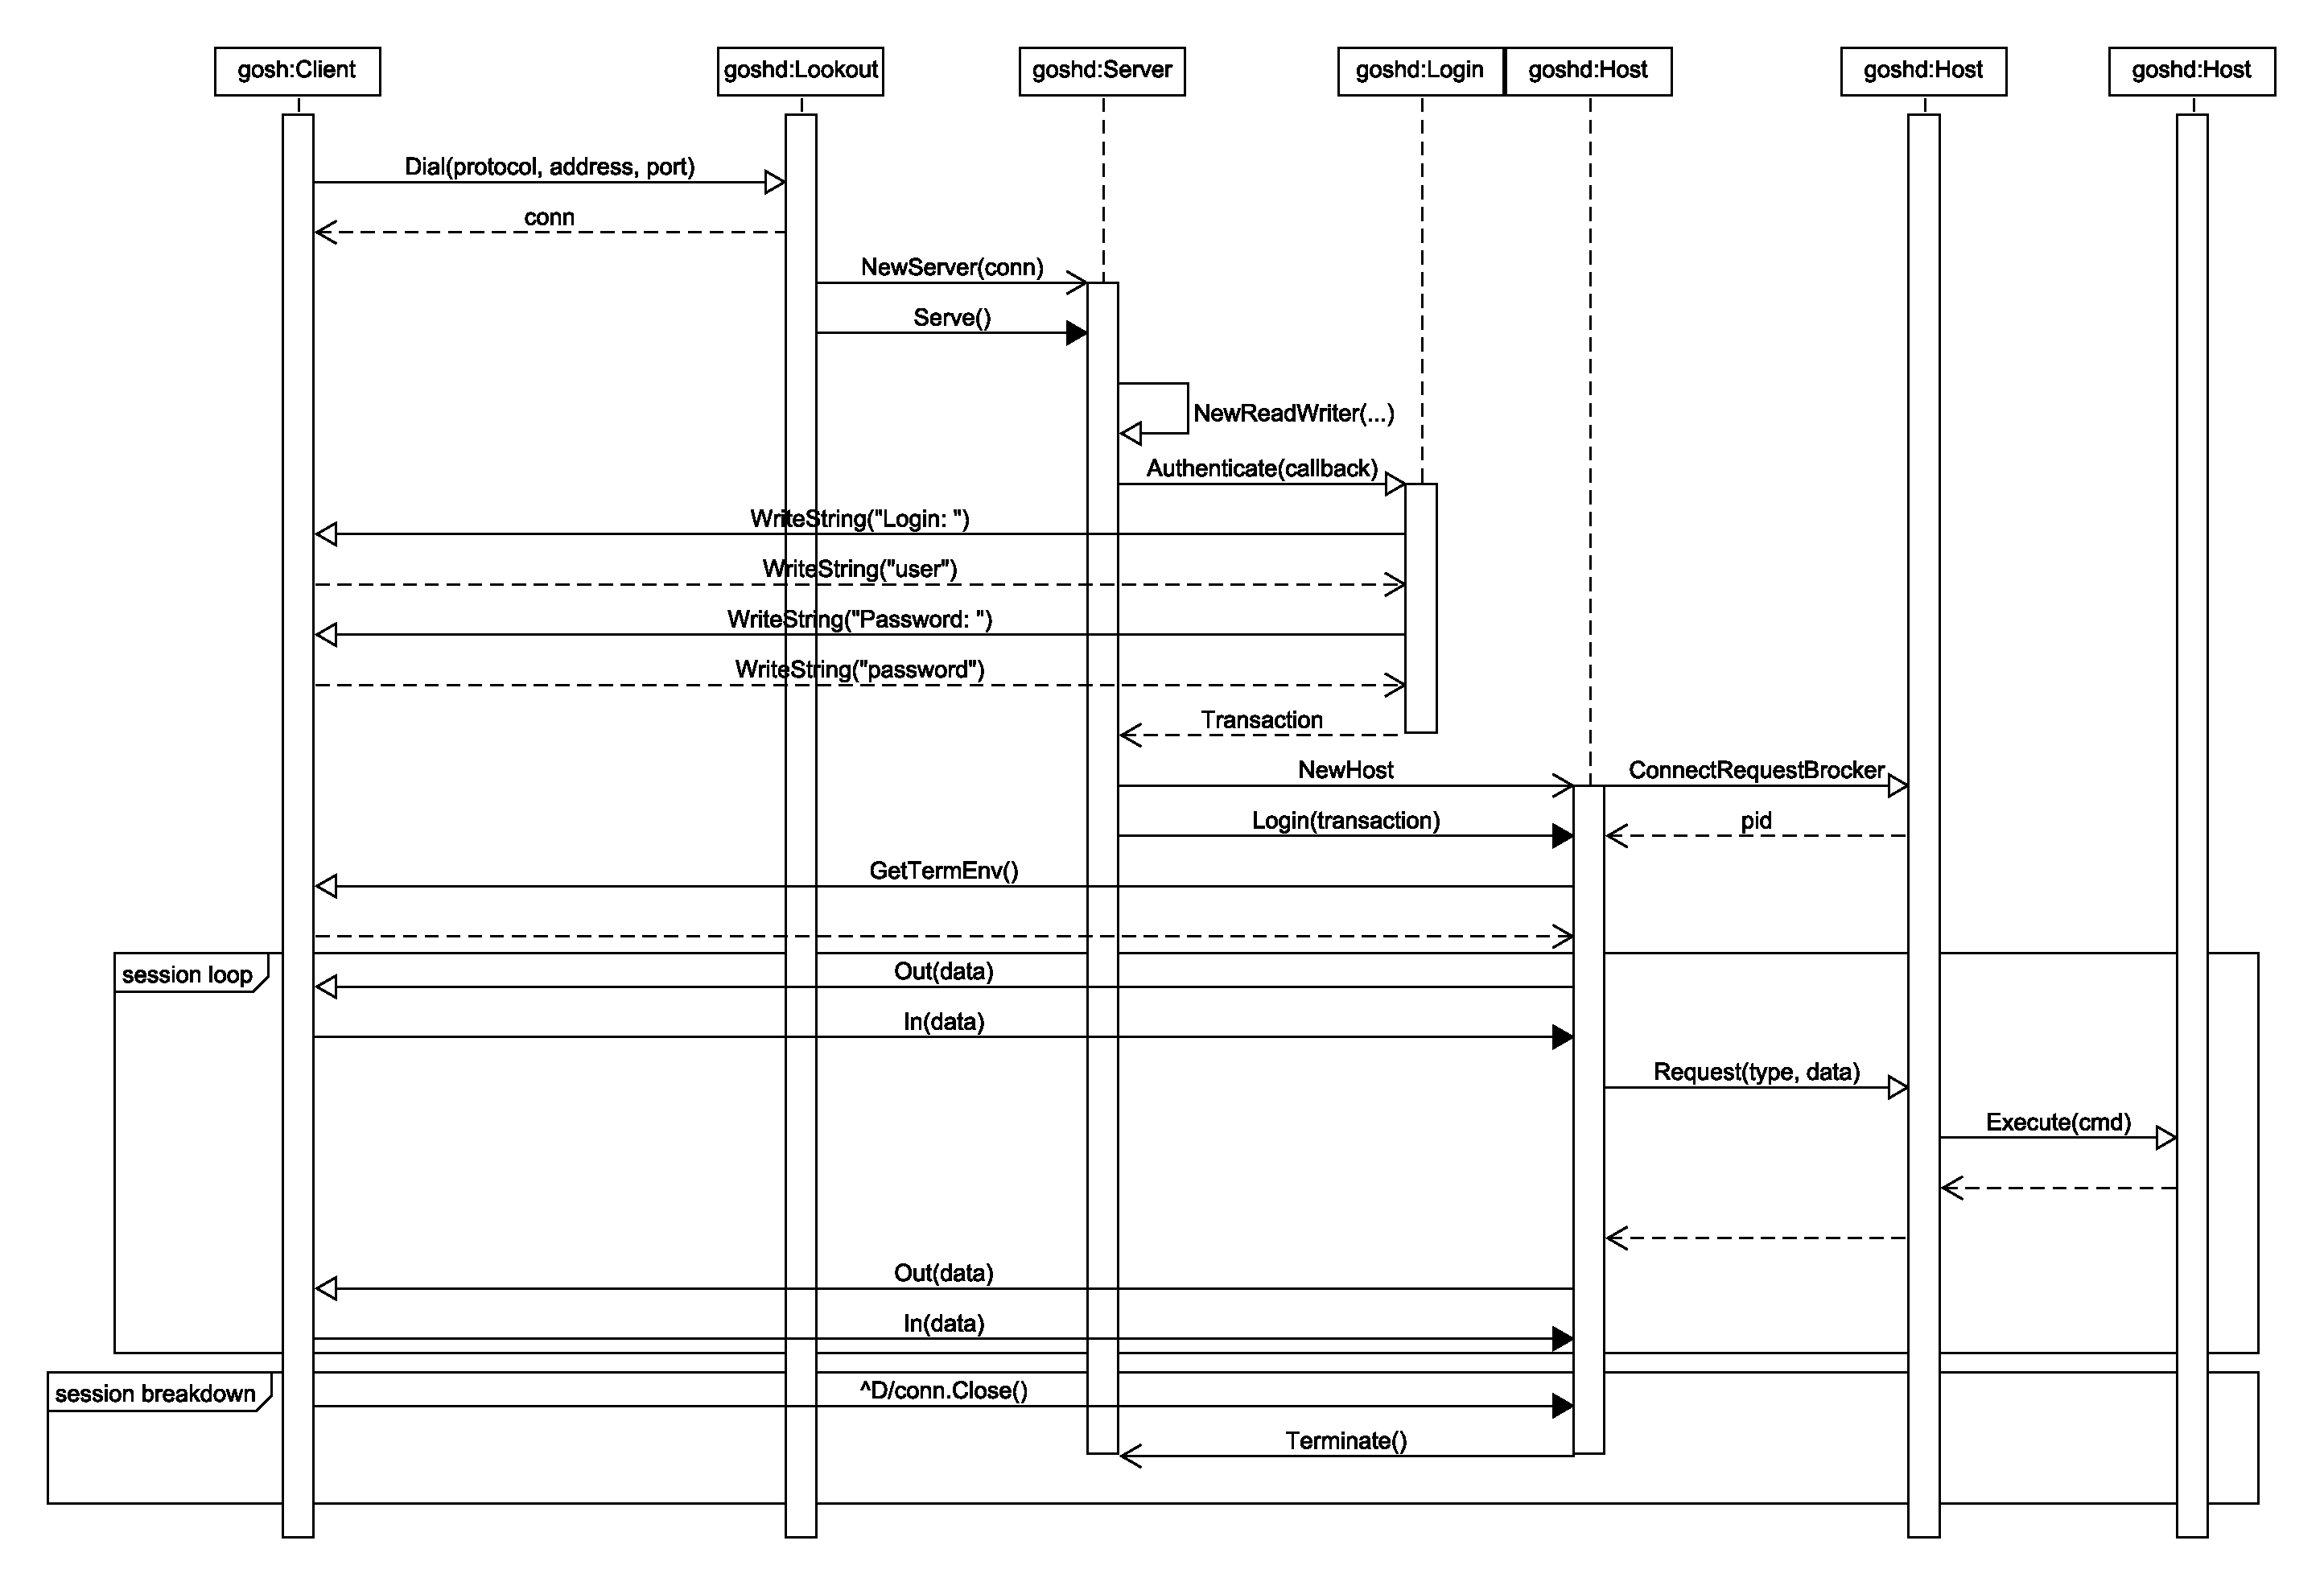
\includegraphics[width=\textwidth]{SequenceDiagram}
\caption{Sequence diagram draft.}
\label{fig:SeqDiaOriginal}
\end{figure}


\section{Implementation Language}\label{sec:DesignImplementationLanguage}
In the beginning of the project, Dr Neuhaus suggested the use of \gls{Go} as a modern low-level language over interpreted languages for considerations of security.
He emphasized that the use of other low-level languages (like \gls{C} or \gls{C++}) was permissible.
In the end the project was implemented in \gls{Go} as suggested.

However, this led to a few problems in the implementation process (See \ref{sec:Problems}).

\section{Secure Connection}\label{sec:DesignSecureConnection}
When building an application that communicates via the network, certain security measures are mandatory to ensure a secure communication.
If such measures are not taken, the communication between the client and the server can be fully read and even altered by a third party.
To prevent this, the communication can be encrypted with \gls{TLS} (originally known as \gls{SSL}).
Today's state-of-the-art is \gls{TLS} 1.3 \citep{rfc8446}.

When connecting, the client checks the server's \gls{X.509}-certificate to authenticate the peer.
Optionally, the client can also authenticate himself to the server.
After this, the two start an encrypted channel by for example using the \gls{DiffieHellmanKX} or letting the server decrypt a random secret that has been encrypted with the servers public key.
After this, every message can be transferred between client and server in an encrypted way.

\section{Authentication via Password}\label{sec:DesignAuthViaPw}
To let a user log in on the system, the user's authenticity has to be proven.
To achieve that, \gls{Linux} provides \gls{PAM}.
It provides a clean separation between a program and the sensitive part of the authentication.
How the server solves this situation is up to the implementation.
It is also possible to rely on the \cite{login} command, which also uses \gls{PAM} in the background.

\section{User Data Querying}\label{sec:DesignUserDataQuerying}
To spawn the default \gls{shell} of a user, the path to said \gls{shell} is required.
This and other information can be found inside the \texttt{/etc/passwd} file.
The file holds information about a user's \gls{login}-\gls{shell}, password hash, groups, user information, \gls{UID}, \gls{GID} and home directory.
To spawn a \gls{shell}, the first and the last of these pieces of information are substantial to successfully log in a user.
To query such data, \gls{Unix} offers \cite{getpw}, which does not just read the \texttt{passwd} file, but also draws information about users from other sources like \gls{NIS} or \gls{LDAP}.


\section{Starting the Shell}\label{sec:DesignStartingTheShell}
A \gls{shell} requires a multitude of information before it can function normally:
\begin{itemize}
\item The name of the user and the host.
\item The \texttt{TERM} variable to allow for the use of \cite{ncurses} dependent applications.
\item The size of the \gls{tty} window (including updates to the window's size).
\item It has to be the session leader.
\end{itemize}

The user information depends on the user that starts the shell or more precisely:
The \gls{UID} and \gls{GID}, with which it has been started.
Note that this is not the same as the display name of the user in the \texttt{USER} variable.
The host name is the same as the \texttt{HOSTNAME} environment variable of the parent process.

There is also to note that for the usage of the correct terminal sequences, the \texttt{TERM} environment variable has to be known to the \gls{shell}.
This is needed to use the correct escape sequences for applications that use \cite{ncurses}.

A \gls{tty} or terminal emulator sends a \gls{SIGWINCH} to its child process to notify a change in its window size.
If this is not forwarded, then the width and size the shell assumes, might collide with the actual values and lead to overflowing lines and unused space.

To take full control of the terminal, the \gls{shell} has to be the session leader.
This can be achieved by letting it set the \gls{SID}.
If it is not set, the \gls{shell} will print some errors regarding the \texttt{ioctl} device.

\section{Login Accounting}\label{sec:DesignLoginAccounting}
When a user logs into a \gls{Unix} machine, a session and a time stamp get created.

For this, the two files \texttt{/var/run/utmp} and \texttt{/var/log/wtmp} provide the appropriate storage.
The \texttt{utmpx} \gls{API} offers appropriate functions.
The \texttt{utmpx} struct represents a single entry in those files:
\setlistingC
\begin{lstlisting}[caption={Definition of the utmpx structure {\citep[p.819]{KerriskTLPI}}},label=lst:UtmpxDefinition]
#define _GNU_SOURCE
/* Without _GNU_SOURCE the two field names below are prepended by "__" */
struct exit_status {
	short e_termination; /* Process termination status (signal) */
	short e_exit; 		 /* Process exit status */
};
#define __UT_LINESIZE 32
#define __UT_NAMESIZE 32
#define __UT_HOSTSIZE 256
struct utmpx {
	short ut_type; 				 /* Type of record */
	pid_t ut_pid; 				 /* PID of login process */
	char ut_line[__UT_LINESIZE]; /* Terminal device name */
	char ut_id[4]; 				 /* Suffix from terminal name, or	ID field from inittab(5) */
	char ut_user[__UT_NAMESIZE]; /* Username */
	char ut_host[__UT_HOSTSIZE]; /* Hostname for remote login, or kernel version for run-level messages */
	struct exit_status ut_exit;  /* Exit status of process marked as DEAD_PROCESS (not filled in by init(8) on Linux) */
	long ut_session; 			 /* Session ID */
	struct timeval ut_tv; 		 /* Time when entry was made */
	int32_t ut_addr_v6[4]; 		 /* IP address of remote host (IPv4 address uses just ut_addr_v6[0], with other elements set to 0) */
	char __unused[20]; 			 /* Reserved for future use */
};
\end{lstlisting}

On \gls{login}, a record has to be written to the \texttt{utmp} file to indicate that the user logged in.
If there is already a record for the active \gls{terminal}, then the entry has to be updated, otherwise a new entry has to be appended.
A call to \cite{pututxline} should suffice in performing these steps properly.
The application has to set the \texttt{ut\_type} field of the \texttt{utmpx} struct to \texttt{USER\_PROCESS} to mark a user \gls{login}.

Similarly to the \texttt{utmp} update after \gls{login}, the application has to report to the \texttt{utmpx} \gls{API} that the session ended.
This procedure consists of almost the same actions as the one after logging in, with exception of \texttt{ut\_user} being zeroed out and \texttt{ut\_type} being set to \texttt{DEAD\_PROCESS}\citep[p.828]{KerriskTLPI}.

A program can also query the \texttt{utmp} file with the according \texttt{get*} methods:
\setlistingC
\begin{lstlisting}[caption={\texttt{utmpx} \gls{API} functions},label=lst:UtmpxApiFunctions]
#include <utmp.h>

struct utmp *getutent(void);
struct utmp *getutid(const struct utmp *ut);
struct utmp *getutline(const struct utmp *ut);

struct utmp *pututline(const struct utmp *ut);
\end{lstlisting}

It is worth mentioning that the \gls{Linux} command \cite{login} also uses PAM to authenticate a user.

\subsection{Login Accounting with PAM}\label{ssec:DesignLoginAccountingWithPAM}
\gls{PAM} supports binding \gls{login} accounting to its own session functions \cite{pam_open_session} and \cite{pam_close_session}:
\setlistingC
\begin{lstlisting}[caption={\gls{PAM} session management},label=lst:PAMSessionManagement]
#include <security/pam_appl.h>

int pam_open_session(pam_handle_t *pamh, int flags);
int pam_close_session(pam_handle_t *pamh, int flags);
\end{lstlisting}

\section{Privilege Separation}\label{sec:DesignPrivilegeSeparation}
Allowing a user to log in as any user requires the authenticating process to have \texttt{root} rights.
However: After performing the authentication procedure and after successfully finishing the latter, a \gls{shell} will be spawned for the user to interact with.
This implies that without dropping the privilege of the process down to the appropriate privileges of the logged in user, the \gls{shell} would run with \texttt{root} rights, which is a privilege escalation and not permissible.

\gls{Linux} provides \cite{setuid} and \cite{setgid} to set the owning user/group of a process and therefore also changing it's permissions.
Unless the user is \texttt{root}, the process' owner cannot be changed.

In comparison: \gls{SSH} chains the authentication of a user between an unprivileged child process that forwards the information between the two processes (see figure \ref{fig:PrivilegeSeparationInSSH}) - thereby putting a privilege separation in place.

\begin{figure}[ht]
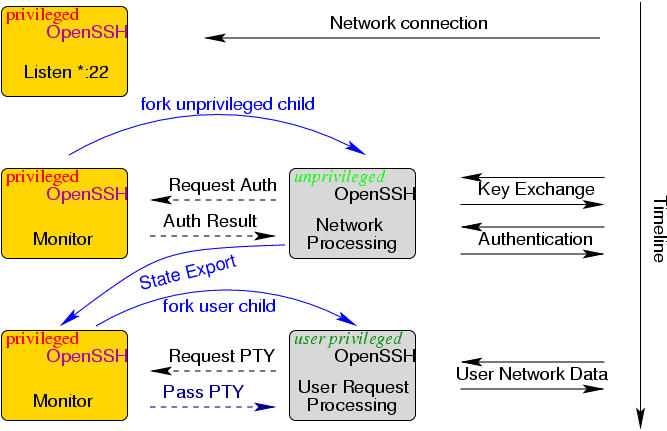
\includegraphics[width=\textwidth]{priv}
\caption{Privilege separation in SSH \citep{ProvosSSHPriv}}
\label{fig:PrivilegeSeparationInSSH}
\end{figure}


\chapter{Implementation}\label{chp:Implementation}
The implementation of the project differs from the envisioned design.
This new version of the server has three executables:

\begin{itemize}
\item The first is the client-side application, that is used to connect to a server.
\item One is \texttt{goshd}, a \gls{daemon} (also refer to \ref{sec:ImplServiceHosting}), which only has one function:
To listen for incoming connections and then to start a child process of the second executable.
\item This last executable is the host (\texttt{goshh}) and it is responsible for handling the new connection.
\end{itemize}

Now, the work flow of the solution looks as follows (note that unchanged entries are \textcolor{gray}{gray}):
\begin{enumerate}
\item \textcolor{gray}{The server listens for incoming connections.}
\item \textcolor{gray}{The client dials server.}
\item The server executes \texttt{goshh} as a child process (referred to as ``host'' in subsequent steps).
\item \textcolor{gray}{The} host \textcolor{gray}{handles the established connection.}
\item \textcolor{gray}{The} host \textcolor{gray}{sets up a secure connection} (see \ref{sec:ImplSecureConnection}).
\item \textcolor{gray}{The} host \textcolor{gray}{requests necessary environment variables from the client.}
\item \textcolor{gray}{The client responds with the values of said variables.}
\item \textcolor{gray}{The} host \textcolor{gray}{notifies the client to prepare itself for the session.}
\item the client sets the appropriate \gls{tty} mode (see \ref{sec:ImplTerminalMode}).
\item \textcolor{gray}{The} host \textcolor{gray}{initiates a \gls{login} procedure}
\begin{itemize}
	\item The host finds a public key that belongs to the client and is authorized for \gls{login} on the specific user account.
	The host now initiates authentication via keys (see \ref{sec:ImplAuthViaKeys}):
	\begin{enumerate}
		\item The host encrypts a random secret with it and then sends that to the client.
		\item The client decrypts the secret and sends the answer back.
		\item The host checks whether the received answer matches the original secret:
		\begin{itemize}
			\item If it matches, the authentication has succeeded.
			\begin{enumerate}
				\item \textcolor{gray}{The} host \textcolor{gray}{gathers essential data about the logged in user} (see \ref{sec:ImplUserDataQuerying}).
				\item \textcolor{gray}{The} host \textcolor{gray}{spawns the users \gls{login} \gls{shell} (see \ref{sec:DesignStartingTheShell}} and \ref{sec:ImplStartingTheShell}\textcolor{gray}{) with the credentials of the logged in user and forwards all traffic between \gls{shell} and client.}
			\end{enumerate}
			\item If it fails, the authentication via keys has failed and instead, the authentication via password gets initiated.
		\end{itemize}
	\end{enumerate}
	\item The host does not find a public key that matches the client or the authentication with keys did not succeed.
	\begin{enumerate}
		\item The host starts an instance of \cite{login}, which asks the client to authenticate itself (see \ref{sec:ImplAuthViaPw}).
		\item After successful \gls{login}, \cite{login} drops privileges, takes post-\gls{login} actions and starts a user \gls{login} \gls{shell}.
	\end{enumerate}
\end{itemize}
\item \textcolor{gray}{The client uses the \gls{shell} on remote machine.}
\item The session ends in particular ways:
\begin{itemize}
	\item \textcolor{gray}{The client terminates session.}
	\begin{enumerate}
		\item The child process of the host terminates.
		\item \textcolor{gray}{The} host \textcolor{gray}{terminates.}
	\end{enumerate}
	\item The client dies.
	\begin{enumerate}
		\item The connection dies.
		\item The \gls{shell} receives \texttt{EOF} and terminates.
		\item \textcolor{gray}{The} host \textcolor{gray}{terminates.}
	\end{enumerate}
	\item The host dies or receives a \gls{SIGINT}.
	\begin{enumerate}
		\item The connection dies.
		\item The client receives \texttt{EOF} and terminates.
	\end{enumerate}
	\item The server dies or receives a \gls{SIGINT}.
	\begin{enumerate}
		\item The server sends a \gls{SIGINT} to all the active hosts.
		\item \textcolor{gray}{The} host \textcolor{gray}{terminates.}
		\item The connection dies.
		\item The client receives \texttt{EOF} and terminates.
	\end{enumerate}
\end{itemize}
\end{enumerate}

A new sequence diagram was created after the rough finishing of the project to display it's new work flow (see figure \ref{fig:SeqDiaCurrent}).

\begin{figure}[ht]
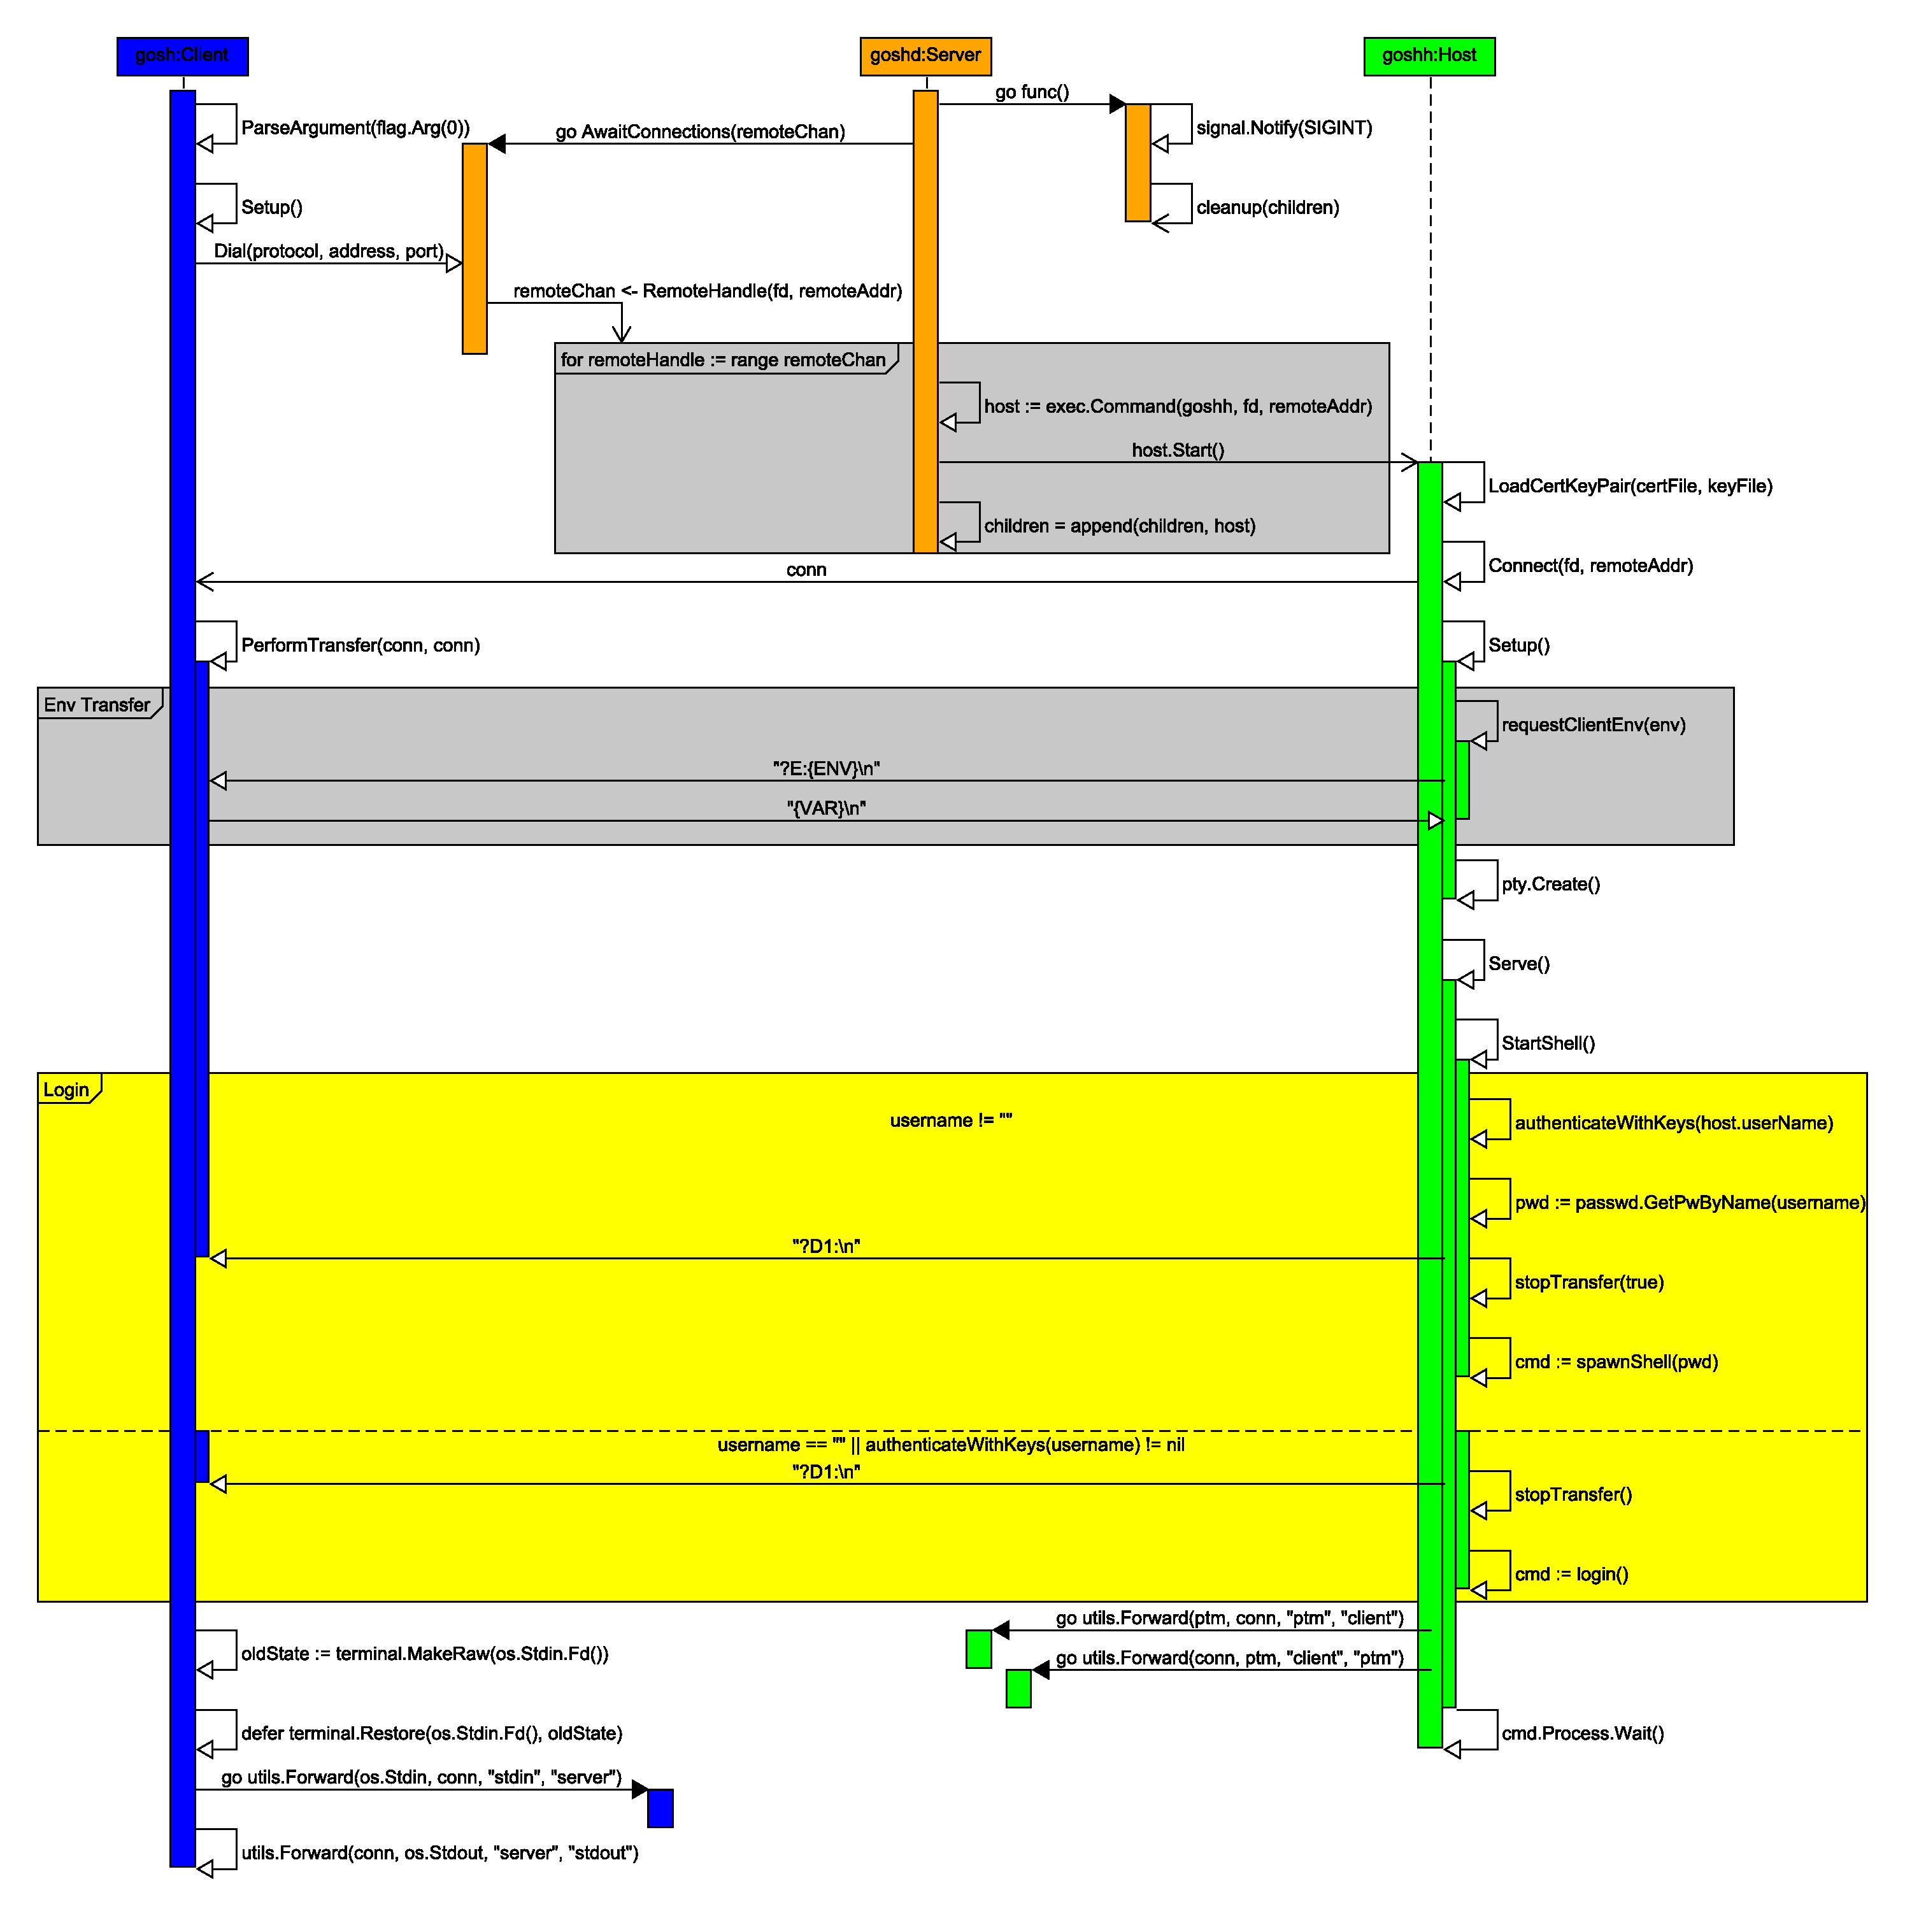
\includegraphics[width=\textwidth]{SequenceDiagramNew}
\caption{Sequence diagram of current implementation.}
\label{fig:SeqDiaCurrent}
\end{figure}

In the process of implementing this project, several problems arose that had to be addressed.
The reason being that some envisioned features or mechanisms could not be implemented as originally thought.
This is also the reason why the work flow described in the beginning of this chapter differs from that of the design in chapter \ref{chp:Design}.

\section{Problems}\label{sec:Problems}
\subsection{Forking}\label{ssec:Forking}
To handle new established connections, it was deemed important to \cite{fork} the process, as this duplicated the current process' memory and returns the \gls{PID}:
0 for the child process and a number greater than 0 for the parent to have the \gls{PID} of the child.

In theory, this should have enabled the program to use \gls{Go}'s standard library capabilities to handle connections.
However, there were several problems with this approach, which break the privilege separation design discussed in section \ref{sec:DesignPrivilegeSeparation}:

\subsubsection{Forking not supported}\label{sssec:ForkingNotSupported}
The \gls{Go} standard library does not support the classical \gls{C}-like forking.
According to Google, \gls{Go} does not have such mechanics, as \gls{Go} was designed with \gls{Go}-routines in mind instead.
\gls{Go}-routines however do not support privilege dropping.
Instead, it only has a \texttt{syscall.ForkExec} method, which is documented as:
\begin{quote}
Combination of \cite{fork} and \cite{exec}, careful to be thread safe.
\end{quote}
But since it uses \cite{exec} as well, it is the same as calling arbitrary binaries/scripts with the \texttt{exec.Cmd} function.

However: \gls{Go} has a feature called \gls{CGo}, which allows programs to call and interact with native \gls{C}-routines.
This opens up the possibility of using \cite{fork}.

\subsubsection{Forking breaks Go objects}\label{sssec:ForkingBreaksGoObjects}
Forking with the functionality of \gls{CGo} does not solve the problem either.
The reason is that after forking there are two programs with a \texttt{net.Conn} object.
This led to both connection objects being corrupted and turning unusable.
Therefore, it was necessary to abandon the clean solution of forking and instead creating a new executable that can handle new connections by its own.

\subsubsection{Sharing Data with Child}\label{sssec:SharingDataWithChild}
The question then was:
How can a process instantiate a child process and hand over all resources to it necessary for handling the new connection?

Since they are two separate processes now, they do not share any memory anymore.
Hence the parent has to give the child the information about the connection via arguments.
The most direct way to deal with this is to use \glspl{fd}, which can be passed as integer arguments to the child.

\subsubsection{Go Connection Cannot Be Transferred}\label{sssec:GoConnectionCannotBeTransferred}
Getting a \texttt{net.Conn} interface from a \gls{fd} is supported in \gls{Go} via:
\setlistingGo
\begin{lstlisting}[caption={Getting a \texttt{net.Conn} interface from a \gls{fd}},label=lst:ConnFromFD]
fd := uintptr(0) // Dummy fd
conn, err := net.FileConn(os.NewFile(fd, "conn"))
if err != nil {
	panic(err.String())
}
\end{lstlisting}

Getting the \gls{fd} from a connection is also possible:
\setlistingGo
\begin{lstlisting}[caption={Getting the \gls{fd} from a \texttt{net.Conn} object},label=lst:FDFromConn]
file, err := conn.(*net.TCPConn).File()
if err != nil {
	panic(err.String())
}
fd := file.Fd()
\end{lstlisting}

However: Creating a connection with the high-level \gls{API} of \gls{Go} and handing over the \gls{fd} to the child to derive a \texttt{net.Conn} object from, fails.

This had some implications for the project:
The listener on the server could not be created with the high-level like:
\setlistingGo
\begin{lstlisting}[caption={\gls{Go}'s high level \gls{API} for listener},label=lst:ListenForConn]
ln, err := net.Listen("tcp", ":8080")
if err != nil {
	// handle error
}
for {
	conn, err := ln.Accept()
	if err != nil {
		// handle error
	}
	go handleConnection(conn)
}
\end{lstlisting}

Instead the project had to rely on the low-level \gls{socket}.
The \gls{x-package} \texttt{Unix} provides the necessary wrapper functions, which can be used instead.

The obvious drawback being having to rely on a \gls{x-package} which is subject to change and not being able to use the higher-level methods which \textbf{are} part of the standard library.

\subsection{Privilege Dropping}\label{ssec:PrivilegeDropping}
To have a sensible privilege separation, the host process should drop the \texttt{root} privileges to the privileges of the logged in user.
But after performing the \gls{login} procedure, setting the \gls{UID} or \gls{GID} both resulted in an error about insufficient permissions.
This problem could not be solved in the course of this project.
Instead, it was relied upon spawning the \gls{shell} already with set \gls{UID} and \gls{GID} values to ensure appropriate permissions.
This worked out well, as looking at the process in a process monitor like \texttt{htop} showed that the spawned \gls{shell} does have the right \gls{UID} and \gls{GID}.

\subsection{Terminal Process Group}\label{ssec:TerminalProcessGroup}
A \gls{login} \gls{shell} such as \texttt{bash} expects a properly set up the \gls{fd} with \cite{ioctl} properly.
This can be done by letting the process set \texttt{ctty}.
However: Setting the corresponding flag when starting the process via \gls{Go} fails with an error.
The solution omits this step, which shows in \texttt{bash} printing the following:

\setlistingBash
\begin{lstlisting}[caption={\texttt{bash} error when starting \gls{shell} without the \texttt{setctty} flag},label=lst:BashIoctlError]
bash: cannot set terminal process group (-1): Inappropriate ioctl for device
bash: no job control for this shell
\end{lstlisting}

\section{Secure Connection}\label{sec:ImplSecureConnection}
As described in \ref{sec:DesignSecureConnection}, \gls{TLS} was used to secure the connection between the client and the server.
For this, the \gls{Go}-package \texttt{crypto/tls} has been used.
This package requires both client and server to extend the \texttt{GODEBUG} variable with a flag to activate support for \gls{TLS} 1.3:
\setlistingGo
\begin{lstlisting}[caption={Activating \gls{TLS} 1.3 in \gls{Go}},label=lst:TlsInGo]
func init() {
    os.Setenv("GODEBUG", os.Getenv("GODEBUG")+",tls13=1")
}
\end{lstlisting}
The server-side of the solution has to have a certificate, which has to be generated newly when actually installing the solution on a machine.
For testing purposes, a self-signed certificate was created using \cite{openssl}:
\setlistingBash
\begin{lstlisting}[caption={Generating a self-signed certificate and private key},label=lst:GenCertNKey]
openssl req -newkey rsa:2048 -nodes -keyout key.pem -x509 -days 365 -out certificate.pem
\end{lstlisting}
The files \texttt{key.pem} and \texttt{certificate.pem} can be found inside the \texttt{test} folder in the project's root folder.

The current implementation is set to skip verification of insecure certificates.
Handling such a case has been decided to be handled in future improvements.
The security aspects of this implementation are discussed in subsection \ref{ssec:SecSecureConnection}.

\section{Authentication via Password}\label{sec:ImplAuthViaPw}
There are no official packages in \gls{Go} that provide a wrapper to \gls{PAM} (refer to \ref{sec:DesignAuthViaPw}).
In earlier stages of the project, a wrapper from \cite{gopam} has been used.
However, \gls{login} using \gls{PAM} failed on one of the test environments (namely Arch \gls{Linux}).
After some trial and error, switching to \cite{login} solved said issue, even though this command also uses \gls{PAM}.
This came with additional desired features like the \gls{login}-accounting and other post-\gls{login} actions (see \ref{sec:DesignLoginAccounting} and \ref{ssec:DesignLoginAccountingWithPAM}), which the command already covers.
After roughly a month of switching to \cite{login}, the \gls{login} procedure failed again on said environment.
This occurred in a later stage of the project and it was deemed to time consuming, returning to the old implementation, which still lacked \gls{login} accounting.
Fortunately this only affected one of the environments:
The other environments (i.e. \gls{WSL}) were still functioning.

\section{Authentication via Keys}\label{sec:ImplAuthViaKeys}
A user can also authenticate himself without a password but instead using public key cryptography.
For this, a user has to create a key pair consisting of a private and a public key.
Before the actual authentication, a hashed version of the public key has to be stored on the server.

When starting an authentication, the user sends his public key to the server, which compares its hash with the stored keys that are deemed permissible for authentication.
If it matches, the server encrypts a random secret (with high entropy) with the public key to the user.
The user decrypts the message with his private key and sends it back to the server.
If the returned secret matches the original secret, the user proved that he is the legitimate owner of the public key.

This authentication is sufficiently secure from third parties which do not have access to the private key of the user, as it can prove the authenticity of a user.

This mechanism has been implemented but with some alterations.

The first change was to store the public key in a plain text format, which was done out of convenience and can be changed in the future.
Not storing the hashed public key does not pose any security threat, so fixing this deviation was deemed of low priority.

The second and last alteration was to have the structure of authorized keys on the server be stored exclusively in the \texttt{root} user's home directory.
This is a sub-optimal approach, as his requires users to store their public keys in the super user's directory, which can lead to mistakes.
This will be fixed in the future.

To test the application, a test user was created and given a key pair which was created as follows using \cite{openssl}:

\setlistingBash
\begin{lstlisting}[caption={Generating a key pair for the client},label=lst:GenClientKeyPair,deletekeywords={in}]
openssl genpkey -out client.pem -algorithm rsa -pkeyopt rsa_keygen_bits:2048
openssl rsa -in client.pem -out client.pub -pubout
\end{lstlisting}

\section{User Data Querying}\label{sec:ImplUserDataQuerying}
Querying user data (see \ref{sec:DesignUserDataQuerying}) is \textit{partially} supported by the \gls{Go} standard library.
It can give all the information about a user on the system but its \gls{login} \gls{shell}.
Therefore it was necessary to obtain said information in a different manner.
One way to get the \gls{login} \gls{shell} of a user is to read in the \texttt{passwd} file of the system.
This originally has been implemented by using a private \gls{Go} package that parsed the \texttt{passwd} file.
This was deemed incomplete, as a system can acknowledge users that are not listed in said file.
An example of this is \gls{NIS} or \gls{LDAP}, which would not be covered by solely relying on the \texttt{passwd} file.

In later stages, this has been corrected by switching to using \gls{CGo} and calling the \gls{Unix} \gls{API} routines \cite{getpw} as described in section \ref{sec:DesignUserDataQuerying}.

\setlistingC
\begin{lstlisting}[caption={Definition of passwd and {\cite{getpw}}},label=lst:PasswdDefinition]
#include <sys/types.h>
#include <pwd.h>

struct passwd {
	char   *pw_name;       /* username */
	char   *pw_passwd;     /* user password */
	uid_t   pw_uid;        /* user ID */
	gid_t   pw_gid;        /* group ID */
	char   *pw_gecos;      /* user information */
	char   *pw_dir;        /* home directory */
	char   *pw_shell;      /* shell program */
};

struct passwd *getpwnam(const char *name);
struct passwd *getpwuid(uid_t uid);
\end{lstlisting}

\section{Starting the Shell}\label{sec:ImplStartingTheShell}
In \gls{Go}, a process can be started with special settings.
These allow for setting the \gls{UID}, \gls{GID} and even letting the process set itself as the session leader.

\setlistingGo
\begin{lstlisting}[caption={Starting a process in \gls{Go}},label=lst:StartingAProcessInGo]
cmd := exec.Command("/bin/bash", "--login")
cmd.SysProcAttr = &syscall.SysProcAttr{
	Setsid: true,
	Credential: &syscall.Credential{
		Uid: pwd.Uid,
		Gid: pwd.Gid,
	},
}
cmd.Env = []string{"TERM=xterm-256color"}
\end{lstlisting}

The transfer of the \gls{SIGWINCH} has not been realized in this project however.


\section{Login Accounting}\label{sec:ImplLoginAccounting}
The current implementation either outsources the post-\gls{login} actions described in \ref{sec:DesignLoginAccounting} to \cite{login}(see \ref{sec:ImplAuthViaPw}) or omits them completely, as is the case in \ref{sec:ImplAuthViaKeys}.
The implementation of this feature is not part of the current project.

\section{Terminal Mode}\label{sec:ImplTerminalMode}
The client expects to send all its input directly to the \gls{shell} without prior interpretation.
To achieve this, the client-side \gls{terminal} has to be set from the default \texttt{cooked}- into the \texttt{raw}-mode\citep[p.1309]{KerriskTLPI}.
This sends each key stroke to the server-side \gls{shell} as is.
After the termination of the session, the original \texttt{cooked}-mode has to be restored to ensure operation as per usual.

Setting the \gls{terminal} mode as described above in \gls{Go} can be achieved with the functionality of the x-package ``\texttt{golang.org/x/crypto/ssh/terminal}'':
\setlistingGo
\begin{lstlisting}[caption={Setting the \gls{terminal} mode in \gls{Go}},label=lst:GoTermMode]
import "golang.org/x/crypto/ssh/terminal"
//...
oldState, err := terminal.MakeRaw(0)
if err != nil {
	panic(err)
}
defer terminal.Restore(0, oldState)
\end{lstlisting}

\section{Pseudoterminal}\label{sec:ImplPseudoterminal}
\glspl{pty} are an \gls{IPC} mechanism that help solving the problem of how two remote programs can communicate as if they were directly connected via a \gls{terminal} (see figure \ref{fig:HowToOperateTtyOrientedProgramOverNetwork}).

A \gls{shell} expects to be connected to a full fledged \gls{tty}(or a \gls{tty} emulator).
To check whether it is inside such an environment, it uses \cite{isatty} on the \gls{fd} it is connected to.
Therefore the \gls{fd} it is connected to should behave like a real \gls{terminal}.
This is where \glspl{pty} come into play.

\begin{figure}[ht]
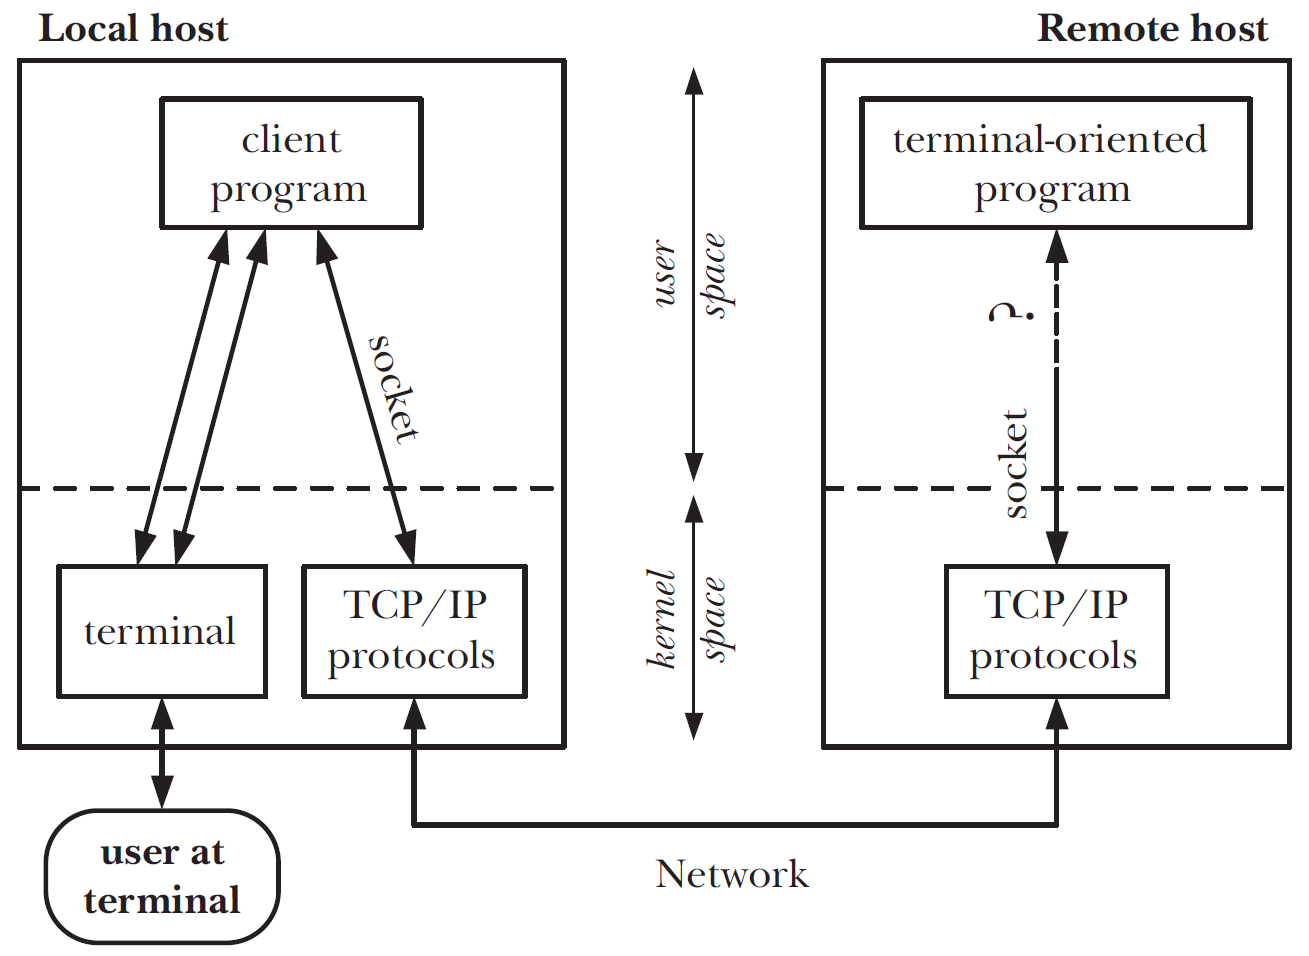
\includegraphics[width=\textwidth]{PseudoterminalProblem}
\caption{How to operate a \gls{tty}-oriented program over a network? \citep[p.1376]{KerriskTLPI}}
\label{fig:HowToOperateTtyOrientedProgramOverNetwork}
\end{figure}

\begin{figure}[ht]
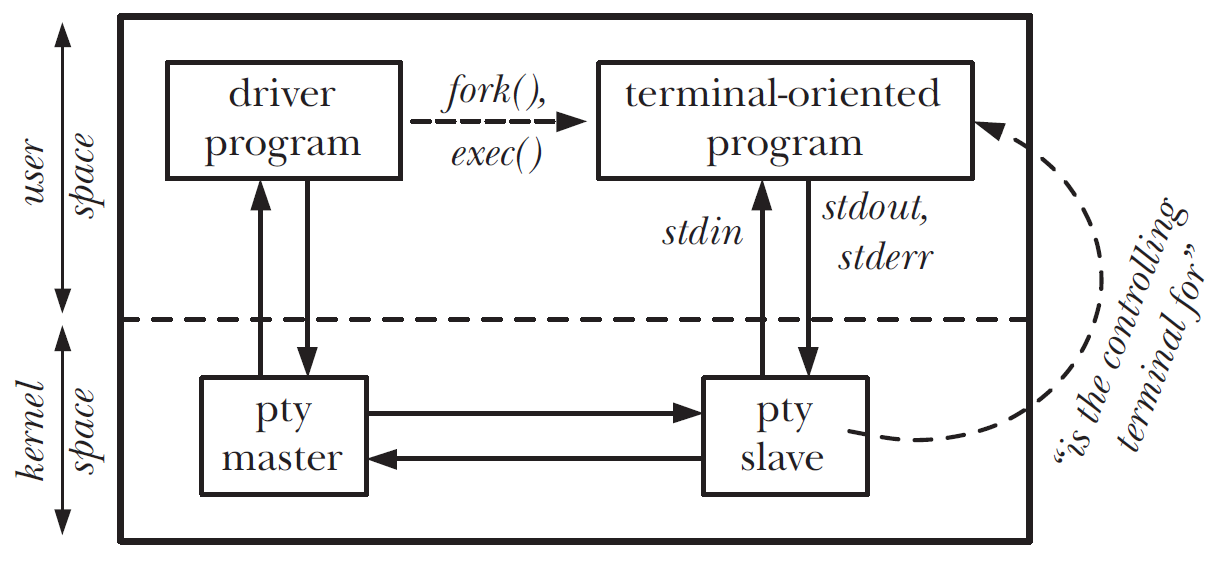
\includegraphics[width=\textwidth]{Pseudoterminal}
\caption{Two programs communicating via a \gls{pty} \citep[p.1377]{KerriskTLPI}}
\label{fig:TwoProgramsCommunicatingViaAPty}
\end{figure}

To do this, two files are created:
The \gls{ptm} and the corresponding \gls{pts}(see figure \ref{fig:TwoProgramsCommunicatingViaAPty}).
\gls{Linux} provides a \gls{pty} generator at \texttt{/dev/ptmx}, which creates a \gls{ptm} and a \gls{pts}.
This works by simply opening the \texttt{/dev/ptmx} file using \cite{posix_openpt}.
After this, a program has to grant the \gls{pts} file ownership and permissions with \cite{grantpt}, unlock it with \cite{unlockpt} and retrieve its file name with \cite{ptsname}:

\setlistingC
\begin{lstlisting}[caption={\gls{pty} related \gls{Linux} \gls{API} functions},label=lst:PtyFunctions]
#define _XOPEN_SOURCE 500
#include <stdlib.h>

int posix_openpt(int flags);
int grantpt(int fd);
int unlockpt(int fd);
char *ptsname(int fd);
\end{lstlisting}

With the \gls{pty} properly set up, a child bound to the \gls{pts} side will assume it is connected to a \gls{terminal} and also behave as such.
This mechanism is key to running a \gls{shell} and forwarding all traffic between a remote client and the \gls{shell}.
In case of \gls{SSH} and the objective of this thesis, the layout looks like in figure \ref{fig:HowSSHUsesPty}.

\begin{figure}[ht]
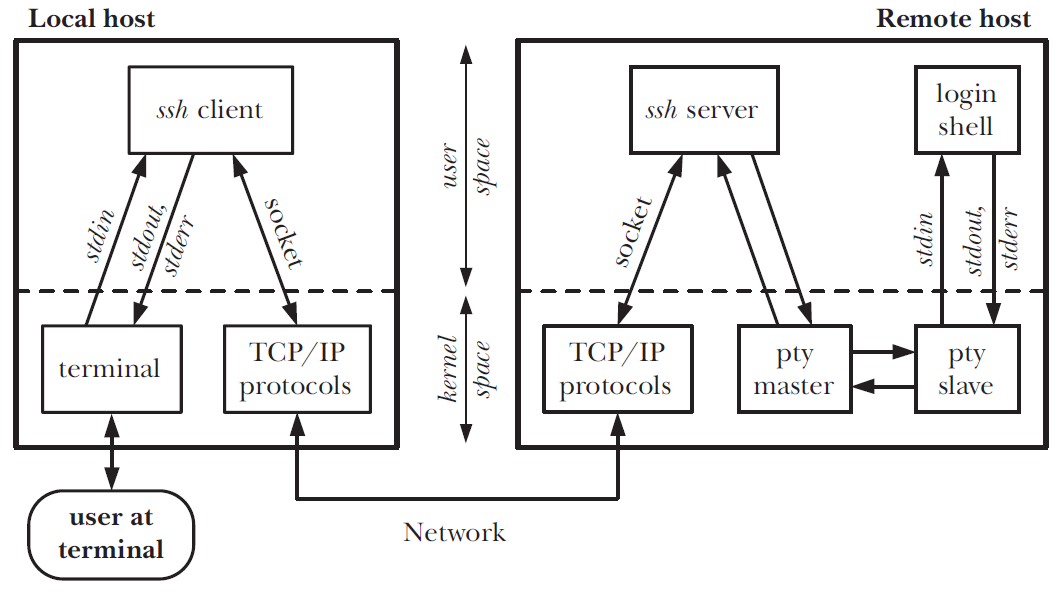
\includegraphics[width=\textwidth]{PseudoterminalSSH}
\caption{How \texttt{ssh} uses a \gls{pty} \citep[p.1378]{KerriskTLPI}}
\label{fig:HowSSHUsesPty}
\end{figure}

\gls{Go} does have a wrapper for \glspl{pty} in an official package, but the code is inside an internal package, called \texttt{os/signal/internal/pty}, which uses \gls{CGo} to call the required \gls{API} routines described in \ref{sec:ImplPseudoterminal}:

\setlistingGo
\begin{lstlisting}[caption={\gls{Go}'s \gls{pty} wrapper},label=lst:GoPty]
// Open returns a master pty and the name of the linked slave tty.
func Open() (master *os.File, slave string, err error) {
	m, err := C.posix_openpt(C.O_RDWR)
	if err != nil {
		return nil, "", ptyError("posix_openpt", err)
	}
	if _, err := C.grantpt(m); err != nil {
		C.close(m)
		return nil, "", ptyError("grantpt", err)
	}
	if _, err := C.unlockpt(m); err != nil {
		C.close(m)
		return nil, "", ptyError("unlockpt", err)
	}
	slave = C.GoString(C.ptsname(m))
	return os.NewFile(uintptr(m), "pty-master"), slave, nil
}
\end{lstlisting}
For the project, this code has been altered to better fit the flow of the application.


\section{Service Hosting}\label{sec:ImplServiceHosting}
The \texttt{goshd} program has to run on a server to accept incoming requests.
For ease of use, the program should be able to be run as a \gls{daemon}.
On \gls{Linux}, this can be achieved using the service manager \cite{systemd}, for which a unit file has been created, which is located inside the \texttt{init} directory of the project.
After deployment of the software, the service can be controlled using \cite{systemd} commands:
\setlistingBash
\begin{lstlisting}[caption={\texttt{goshd} service control},label=lst:GoshdServiceCtl,deletekeywords={enable}]
# Setup of goshd
sudo systemctl enable goshd.service
sudo systemctl start goshd.service
sudo systemctl info goshd.service

# Breakdown of goshd
sudo systemctl stop goshd.service
sudo systemctl disable goshd.service
\end{lstlisting}


\chapter{Results}\label{chp:Results}
% (Zusammenfassung der Resultate)
\begin{figure}[ht]
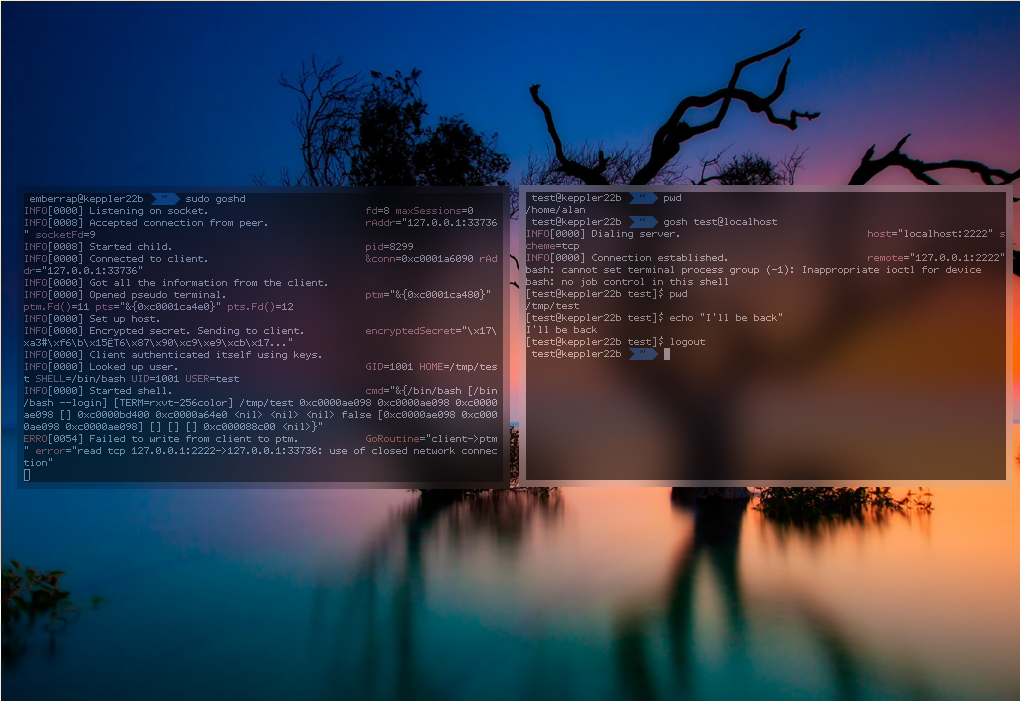
\includegraphics[width=\textwidth]{ohmygosh}
\caption{Screenshot of \texttt{gosh} (right) connecting to the local \texttt{goshd} (left) server.}
\label{fig:OhMyGoshScrot}
\end{figure}

The project provides 3 applications:
\begin{itemize}
\item \texttt{gosh} is the application for the client side use case.
It takes the following arguments:
\begin{itemize}
\item \texttt{--help}: Displays the help text.
\item \texttt{--conf}: Sets the path where the configuration file is stored (defaults to ``\texttt{/etc/gosh}'').
\item \texttt{--auth}: Sets the path where the key pair is stored (defaults to ``\texttt{~/.gosh}'').
\item \textit{string}: An optional address with optional credentials (defaults to \texttt{localhost}).
\end{itemize}
\item \texttt{goshd} is the \gls{daemon} on the server side that awaits incoming requests.
It takes the following arguments:
\begin{itemize}
\item \texttt{--help}: Displays the help text.
\item \texttt{--conf}: Sets the path where the configuration file is stored (defaults to ``\texttt{/etc/gosh}'').
\item \texttt{--auth}: Sets the path where the key pair is stored (defaults to ``\texttt{~/.gosh}'').
\item \texttt{--cert}: Sets the path of the server certificate (defaults to ``\texttt{/etc/gosh/certifi\linebreak{}cate.pem}'').
\item \texttt{--key}: Sets the path of the server key file (defaults to ``\texttt{/etc/gosh/key.pem}'').
\end{itemize}
\item \texttt{goshh} is a host that handles a new connection.
This binary is only executed by the server and takes the following arguments:
\begin{itemize}
\item \texttt{--help}: Displays the help text.
\item \texttt{--conf}: Sets the path where the configuration file is stored (defaults to ``\texttt{/etc/gosh}'').
\item \texttt{--auth}: Sets the path where the key pair is stored (defaults to ``\texttt{~/.gosh}'').
\item \texttt{--cert}: Sets the path of the server certificate (defaults to ``\texttt{/etc/gosh/certifi\linebreak{}cate.pem}'').
\item \texttt{--key}: Sets the path of the server key file (defaults to ``\texttt{/etc/gosh/key.pem}'').
\item \texttt{--remote}: Sets the address of the peer (defaults to ``\texttt{localhost:2222}'').
\item \texttt{--fd}: Provides the \gls{fd} of the connection the host has to handle.
\end{itemize}
\end{itemize}

To configure the applications, the client side has a configuration file called \texttt{gosh\_config.toml}.
The server's configuration file is called \texttt{goshd\_config.toml} respectively, where both \texttt{goshd} and \texttt{goshh} refer to the same file.
In it, the user can specify the following parameters and a few more:
\begin{itemize}
\item The default port to communicate over.
\item The default log level.
\item The location of the authorized keys.
\item The maximum amount of allowed sessions (server-side only).
\end{itemize}

The project allows a user to connect to a server and enter an interactive session with a remote user's \gls{login} \gls{shell} (see \ref{sec:ImplTerminalMode}, \ref{sec:ImplAuthViaPw}, \ref{sec:ImplAuthViaKeys}, \ref{sec:ImplPseudoterminal} and \ref{sec:ImplLoginAccounting}).
On the server side an appropriate privilege separation is performed upon user \gls{login} (see \ref{sec:DesignPrivilegeSeparation} and \ref{sec:Problems}).
The communication is secured in the beginning of the transaction using \gls{TLS} (see \ref{sec:ImplSecureConnection}).

To test the applications, the user can execute the binaries from within the root folder of the project on both the client and the server (they can be the same machine, if so desired).
To do this, the user can make use of the \gls{CLI} flags described above to redirect the dependencies to the test files in the project:
\setlistingBash
\begin{lstlisting}[caption={Running the applications for test purposes},label=lst:RunProject,deletekeywords={test}]
# Setup environment: Create test user, its home directory and the login shell.
./scripts/setup.sh

# Start the server
sudo goshd --conf configs --auth test --cert test/certificate.pem --key test/key.pem

# Start the client
gosh --conf configs --auth test
# Or
gosh --conf configs --auth test 192.168.0.100
# Or
gosh --conf configs --auth test test@localhost
\end{lstlisting}

To change the log level, giving the application the environment variable \texttt{LOG\_LEVEL} set to the desired log level (i.e. ``trace'', ``debug'', etc.) should suffice.

\chapter{Discussion And Prospects}\label{chp:DiscussionAndProspects}
% Bespricht die erzielten Ergebnisse bezüglich ihrer Erwartbarkeit, Aussagekraft und Relevanz
% Interpretation und Validierung der Resultate
% Rückblick auf Aufgabenstellung, erreicht bzw. nicht erreicht
% Legt dar, wie an die Resultate (konkret vom Industriepartner oder weiteren Forschungsarbeiten; allgemein) angeschlossen werden kann; legt dar, welche Chancen die Resultate bieten
As described in chapter \ref{chp:Results}, the developed solution is capable of providing a \gls{TLS} secured channel to an interactive session of a remote user's \gls{shell}, of which the privilege has been dropped to the appropriate level for said user.
It can be said that with this, the main goal of this thesis could be achieved.
In the following list, an overview of the solutions to the official tasks are given and explained:
\begin{itemize}
\item \textbf{Design and implement a client-server protocol that can manage interactive sessions}

This has been completed in chapters \ref{chp:Design} and \ref{chp:Implementation} respectively.
Both chapters give an overview and then list certain points of interest to be highlighted.

\item \textbf{Design and implement a privilege-separation architecture on the server side that allows safe dropping of privileges once a client establishes a connection}

The design has been discussed in section \ref{sec:DesignPrivilegeSeparation} and the implementation and problems encountered displayed in subsection \ref{ssec:PrivilegeDropping} respectively.
Despite the encountered problems, a privilege separation was still realized.
\end{itemize}

As described in section \ref{sec:Task}, the following tasks are required for a passing grade:

\begin{itemize}
\item \textbf{An introduction to the problem and why the envisaged solution will solve it}

This has been discussed in chapter \ref{chp:Introduction}.

\item \textbf{A survey of related work in the area}

Related works are listed and discussed in chapter \ref{chp:Introduction} as well (specifically in the sections \ref{sec:OpenSSH}, \ref{sec:Telnet} and \ref{sec:BerkeleyRCommands}).

\item \textbf{A detailed design of the solution}

The entire design can be found in chapter \ref{chp:Design}.
The implementation differs from the original design however, which is also discussed in chapter \ref{chp:Implementation}.

\item \textbf{An evaluation of the performance of the implemented solution}

% TODO: Write more
An explanation to this task can be found at subsection \ref{sec:Performance}.

\item \textbf{A privilege-separation architecture}

This is the same as the first task and can be considered solved as of section \ref{sec:DesignPrivilegeSeparation} with remark to subsection \ref{ssec:PrivilegeDropping}.
\end{itemize}

In the following lists, there are additional tasks described in section \ref{sec:Task}:

\begin{itemize}
\item \textbf{A comparison of all the related work with the envisaged solution, outlining why the envisaged solution is better}

A small comparison to the surveyed solutions can be found in section \ref{sec:Comparison}.

\item \textbf{A detailed analysis of the security of the solution, including
possible attacks and defenses}

This task will be cleared later in this chapter: The section \ref{sec:Security} clears this task.

\item \textbf{Use of TLS as the transport layer}

This topic can also be considered solved as of sections \ref{sec:DesignSecureConnection} and \ref{sec:ImplSecureConnection}.

\item \textbf{A proof-of-concept client that can handle interactive sessions}

A usable client has been developed and can be used after compilation of the source code.
An overview of the developed applications can be found in chapter \ref{chp:Results}.

\item \textbf{A proof-of-concept client that works as a transport for rsync}

This is a task that has not been solved in this thesis but its addition is discussed in subsection \ref{ssec:Rsync}.
\end{itemize}



\section{Performance}\label{sec:Performance}
The \gls{pty} is an interface that needs data to be forwarded to and received from.
This holds true for both sides (\gls{ptm} and the \gls{pts}) and therefore needs a mechanism to transfer said data.
On the slave side, the \gls{shell} itself already seamlessly communicates with the device via its standard pipes.
A similar concept is applied for the client and its connection to the server, where the application communicates via the connection with the server.
There, the client uses a \gls{Go}-routine to asynchronously forward the standard input of the program to the connection.

The master side has to transfer the input from the remote client to the \gls{ptm} and the output from the latter to the former as well.
For this, the server uses two \gls{Go}-routines that asynchronously forward the data from each stream to the other and waits until the shell process terminates.

Both these transfers are performed using \gls{Go}'s \texttt{WriteTo} method:
\setlistingGo
\begin{lstlisting}[caption={\texttt{WriteTo} method of \gls{Go}},label=lst:GoWriteTo]
// WriteTo implements io.WriterTo.
// This may make multiple calls to the Read method of the underlying Reader.
// If the underlying reader supports the WriteTo method,
// this calls the underlying WriteTo without buffering.
func (b *Reader) WriteTo(w io.Writer) (n int64, err error)
\end{lstlisting}

This mechanism helps keeping the memory usage low.

As for speed, the application has been tested on speed of the connection.
For this, the client was changed to sending a stream of zeroes from \texttt{/dev/zero} to the connection once the latter has been established.
The server-side on the other hand still spawns a \textit{host}, but that forwards the entire data received from the connection to its \texttt{stdout}.
To measure the throughput, the server's output gets piped into pipeviewer (\texttt{pv}), with the following arguments:
\begin{itemize}
\item \texttt{-t}: show elapsed time
\item \texttt{-r}: show data transfer rate counter
\item \texttt{-a}: show data transfer average rate counter
\item \texttt{-b}: show number of bytes transferred
\item \texttt{-W}: display nothing until first byte transferred
\end{itemize}
The data stream gets then redirected to \texttt{/dev/null}.

\setlistingBash
\begin{lstlisting}[caption={Throughput measurement},label=lst:ThroughputMeasurement]
# Set the log level to error to prevent sending bytes to pv before the client sends the stream
sudo LOG_LEVEL=error goshd | pv -rabtW > /dev/null
\end{lstlisting}

Two variations of the test were performed:
One using the blank \gls{Go} connection \texttt{net.Conn} and the other one having a \gls{TLS} layer in between.
The equipment for this test consisted of a native Arch \gls{Linux} laptop and an Ubuntu \gls{Linux} running inside a native Window's \gls{WSL}.

Using this as a basic setup, several tests were performed:
\begin{itemize}
\item On a native Arch \gls{Linux} laptop, the whole solution was tested over \gls{loopback}.
\item Similarly, the solution was also tested over \gls{loopback} in \gls{WSL}.
\item Connected via a switch, \gls{WSL} hosted the server.
The same Arch \gls{Linux} laptop as in the former test connected to the server as the client.
\end{itemize}

All the runs were performed for exactly one minute.
The measured speeds are as follows:
\begin{table}[ht]
\centering
\begin{tabular}{rcc}
&\gls{TLS} (size) & no \gls{TLS} (size)\\\hline
Arch \gls{Linux} (\gls{loopback}) 			& 427 MiB/s (25.1 GiB) & 1.15 GiB/s $\simeq$ 1177.6 MiB/s (69.0 GiB)\\
\gls{WSL} (\gls{loopback}) 					& 69.7 MiB/s (4.09 GiB) & 116 MiB/s (6.82 GiB)\\
Arch \gls{Linux} to \gls{WSL} (ethernet) 	& 85.1 MiB/s (4.99 GiB) & 83.7 MiB/s (4.91 GiB)
\end{tabular}
\caption{Throughput measurements}
\label{tbl:}
\end{table}

The throughput in \gls{WSL} never deviated by more than 8 MiB/s, whereas Arch \gls{Linux} had deviations in the scale of 0.3.
A reason for this was not found.
The reason for the comparably low throughput over a network, however, was assumed to be the combination of the Netgear switch and a Cat 5 ethernet cable.

This demonstrates that the application is sufficiently fast to be used in most use cases.
Therefore the feature of this solution to be used as a transport protocol (i.e. for \cite{rsync} - see \ref{ssec:Rsync}) is deemed viable.


\section{Comparison}\label{sec:Comparison}
\subsection{OpenSSH}\label{ssec:CompOpenSSH}
As described in section \ref{sec:OpenSSH}, \gls{SSH} uses an own protocol to secure the connection between client and server.
This project differs in this point, as it uses \gls{TLS} to create a secure channel (see \ref{sec:DesignSecureConnection} and \ref{sec:ImplSecureConnection}).

Both \gls{SSH} and the developed solution provide means to login with a user/password combination or via keys.
This feature behaves the same in both cases.

\gls{SSH} has a plethora of features that are not supported by the solution, but also were not required.
The reason for that is simply because the task was to create a simple alternative.

Both have privilege separation mechanisms implemented, but the developed solution was not able to drop the privilege of the host process after \gls{login}.
This is another point where the two differ.
That the solution does not drop privileges after \gls{login} is also listed as a security issue in section \ref{sec:Security}.

Authentication in \gls{SSH} are per default solved using \gls{PAM}, which can be changed in the configuration files.
Although the project in earlier stages used \gls{PAM} as well, it outsourced the \gls{login} functionality to \cite{login}, which in turn uses \gls{PAM} as well.

\gls{SSH} also performs \gls{login} accounting in each case, whereas the solution again outsources this mechanism to \cite{login} or omits it completely (in the case of authentication via keys).
This is a feature that is missing from the project (see \ref{ssec:UsingUtmpx}).

\subsection{Telnet}\label{ssec:CompTelnet}
In comparison to \cite{telnet}, the solution has several differences, that distinguishes it from the old protocol.
For one, the communication channel of \cite{telnet} is not secured.
The developed solution however provides a \gls{TLS} secured communication tunnel.
This is the main difference between these two.

Furthermore, \cite{telnet} does not support authentication via keys, which is a feature that has been implemented in the project.
Authentication via keys is also performed using \gls{PAM}.

Just as in the case of \gls{SSH}, it also does proper \gls{login} accounting, which as mentioned before is missing in the solution when authenticating via keys.

\subsection{Berkeley r-Commands}\label{ssec:BerkeleyRCommands}
From the list of Berkeley r-commands, only \cite{rlogin} is of interest, as the other ones are used with slightly different use cases in mind.
The only other one that could be compared to as well is \cite{rsh}, which without a command to execute on the remote server behaves the same as \cite{rlogin}.

As mentioned in section \ref{sec:Telnet}, the communication channel of \cite{rlogin} is not secured.
Just as with \cite{telnet}, user-password combinations are sent over a network in plain text and can be read without much difficulty.
This gets prevented in the developed solution by relying on \gls{TLS}.

The r-commands also do not support authentication via keys, which has been implemented in the solution.
The authentication via password on the other hand is virtually the same, as both use \cite{login} to accomplish this task.
This also goes for using \gls{PAM} for authentication, \gls{login} accounting and the post-\gls{login} actions the server performs.


\section{Security}\label{sec:Security}
Although the solution uses \gls{TLS} as a security measure, the current state of the project still has several weaknesses.
Some of them seem to be of a lower magnitude, whereas others have a higher priority to be resolved.
This section lists some security issues that have been solved and others that are still unsolved.

\subsection{Secure Connection}\label{ssec:SecSecureConnection}
A secure channel is mandatory in an architecture like this.
As described in sections \ref{sec:DesignSecureConnection} and \ref{sec:ImplSecureConnection}, the connection has been secured using \gls{TLS} (specifically \gls{TLS} 1.3).
This means an attacker has to deal with the security measures that \gls{TLS} brings with itself.

Apart from that, the current solution only uses a server-side certificate;
The client's certificate is never checked as it does not exist in the current solution.
This means an attacker that knows the \gls{login} credentials of a user on the remote system can log in in the system and deal harm to it without the server being able to distinguish the attacker machine from the expected client.
Using client-side certificates could help to increase the level of difficulty of an attacker to perform this attack.

Furthermore, in the current solution, insecure server certificate errors simply get ignored.
An attacker can use this to take on the role of a ``man in the middle''.
This attack vector allows the attacker to appear to the client like it is the server the client wants to log in to and at the same time appear to the server as if it is the client trying to connect to it.
This leads to two \gls{TLS} connections:
One from the client to the attacker and one from the attacker to the server.
This means the attacker can read the entire data stream in an unencrypted way and manipulate as desired.
This also leads to possible password exposure to the attacker if the client authenticates itself via password to the server.
Therefore this weakness is considered a severe security issue that can easily be exploited by an attacker by simply sitting between the two connecting parties.
To prevent such attacks, the certificate verification cannot be skipped.


\subsection{Authentication}\label{ssec:SecAuthentication}
As described in sections \ref{sec:DesignAuthViaPw}, \ref{sec:ImplAuthViaPw} and \ref{sec:ImplAuthViaKeys}, two possible paths of authentication were realized.

\subsubsection{Authentication via Password}\label{sssec:SecAuthViaPw}
Relying on \cite{login} simplified the task, as time was pressing.
Using this standardized command also helps removing possible security issues in the authentication process and afterwards.
However, this comes with a cost:
The \cite{login} command allows a user to directly log in as \texttt{root} user.
This cannot be prevented by the server.
Ideally the server would have a default option of allowing root login set to false.
There is no reason to allow any client to try to log in as \texttt{root} user.
Especially since a logged in user can simply use \texttt{su} or \texttt{sudo} to gain \texttt{root} privileges.
``\texttt{root}'' however is the only user name that can be logged in and an attacker knows exists and only needs the knowledge of one password (which \textit{could} be a default password) to gain full system control.

Another way to prevent \texttt{root} user login despite the usage of \cite{login} could be to pre-fetch the user credentials from the client (see \ref{ssec:PrefetchingOfCredentials}).

\subsubsection{Authentication via Keys}\label{sssec:SecAuthViaKeys}
When authenticating a user via public key cryptography, the server looks up which users can be logged in.
It does so by looking into the \texttt{root} user's home directory \texttt{/root/.gosh}.
There, the directory structure defines what public key can log in as which user.
In this case, Each directory has the name of a user and inside are the public keys stored in plain text with the file name of the \texttt{USER} value of the connecting client.
This for one means that to allow a remote user to log in as this very user, the remote user's public key has to be named after that user's name and placed into the \texttt{root} user's home directory.
Storing such files in the \texttt{root} user's home directory is a bad idea as this means that every change to this file structure needs \texttt{root} privileges.
The public keys are also stored in plain text, which is not needed and can be replaced with their hashes instead as described in section \ref{sec:ImplAuthViaKeys}.

\subsection{Privilege Separation}\label{ssec:SecPrivilegeSeparation}
To have a proper privilege separation (see section \ref{sec:DesignPrivilegeSeparation}), the host process should also drop its privileges once the \gls{login} succeeded.
This is desired as the forwarding of the data is still in the host's hands and as the host still runs with \texttt{root} privileges, an attacker could potentially gain \texttt{root} access if the attacker manages to gain access to that process.
Such privilege escalation should be prevented but was not entirely achieved in the current solution, as described in subsection \ref{ssec:PrivilegeDropping}.


\section{Prospects}\label{sec:Prospects}
Although the project created a working alternative to \gls{SSH}, there are several points that have to be improved, which couldn't be completed in the course of this thesis.
These points are listed here:

\subsection{Security Issues}\label{ssec:SecurityIssues}
Of course the primary task to solve in further works would be to solve the security issues with this project.
As this project should be able to replace \gls{SSH} in its core functions, the security aspects have to be comparable as well.
Suggestions on how to solve the above mentioned security issues can be found in the respective subsections \ref{ssec:SecSecureConnection}, \ref{ssec:SecAuthentication} and \ref{ssec:SecPrivilegeSeparation}.

\subsection{Rsync}\label{ssec:Rsync}
One of the proposed extensions was to use this project's solution as a transport layer for \cite{rsync}.
This could not be achieved in the course of this project, but could be done in subsequent works.

\subsection{Prefetching of Credentials}\label{ssec:PrefetchingOfCredentials}
Instead of forwarding the client's inputs to the \gls{login} mechanism, the client could ask the user for user name and password beforehand and send them to the server.
The server can then check for the user name to be sane (for example for preventing \texttt{root} login) and only then forward it to \cite{login}.
This could solve the security issue discussed in subsection \ref{ssec:SecAuthentication}.

\subsection{Using PAM}\label{ssec:UsingPAM}
In earlier stages of the project the authentication via password was already partially solved by using \gls{PAM}.
For other reasons (see \ref{sec:ImplAuthViaPw}) this was dropped in favor of \cite{login}.
It is suggested to return to using \gls{PAM} directly and also handle \gls{login} accounting (see \ref{sec:DesignLoginAccounting}) as well.

\subsection{Using Utmpx}\label{ssec:UsingUtmpx}
Part of post-\gls{login} actions are \gls{login} accounting, which would be realized using \gls{Linux}' \texttt{utmpx}-\gls{API}.
This does happen in the case of relying on \cite{login}, but not in the case of authentication via keys.
The session is therefore not properly set up and should be added in future works.

\subsection{Add Transfer of SIGWINCH}\label{ssec:AddTransferOfSIGWINCH}
As mentioned in section \ref{sec:ImplStartingTheShell}, the \gls{SIGWINCH} is not being transferred to the \gls{shell}.
This means that the \gls{shell} assumes default values for window width and height, which leads to faulty formatting.
This feature should be implemented to make the interactive session more seamless.

\subsection{Forwarding of Data Flow}\label{ssec:ForwardingOfDataFlow}
As of now, the solution simply calls forwarding routines to transfer the data flow between the \gls{shell} (of more specifically, the \gls{ptm}) and the connection to the client.
This sometimes leads to an unclean session breakdown when terminating.
It is therefore desirable to implement the data forwarding with other means.
Possible \gls{Linux} support could be drawn from the functions \cite{select} or \cite{poll}.


\chapter{Index}\label{chp:Index}
\bibliography{reference}\label{sec:Bibliography}
\newpage
\printglossary\label{sec:Glossary}
\newpage
\listoffigures\label{sec:ListOfFigures}
\newpage
%\listoftables\label{sec:ListOfTables}
%\newpage
\lstlistoflistings\label{sec:ListOfListings}
\newpage
\printglossary[title=SymbolGlossary,type=symbols]\label{sec:SymbolGlossary}
\newpage
\printglossary[title=Acronym Glossary,type=\acronymtype]\label{sec:AcronymGlossary}
\newpage
\printindex\label{sec:Index}

\appendix
\chapter{Appendix}\label{chp:Appendix}
\section{Project Management}\label{sec:ProjectManagement}
% Offizielle Aufgabenstellung, Projektauftrag
% (Zeitplan) 
% (Besprechungsprotokolle oder Journals)

\subsection{Official Statement of Tasks}\label{ssec:OfficialStatementOfTasks}
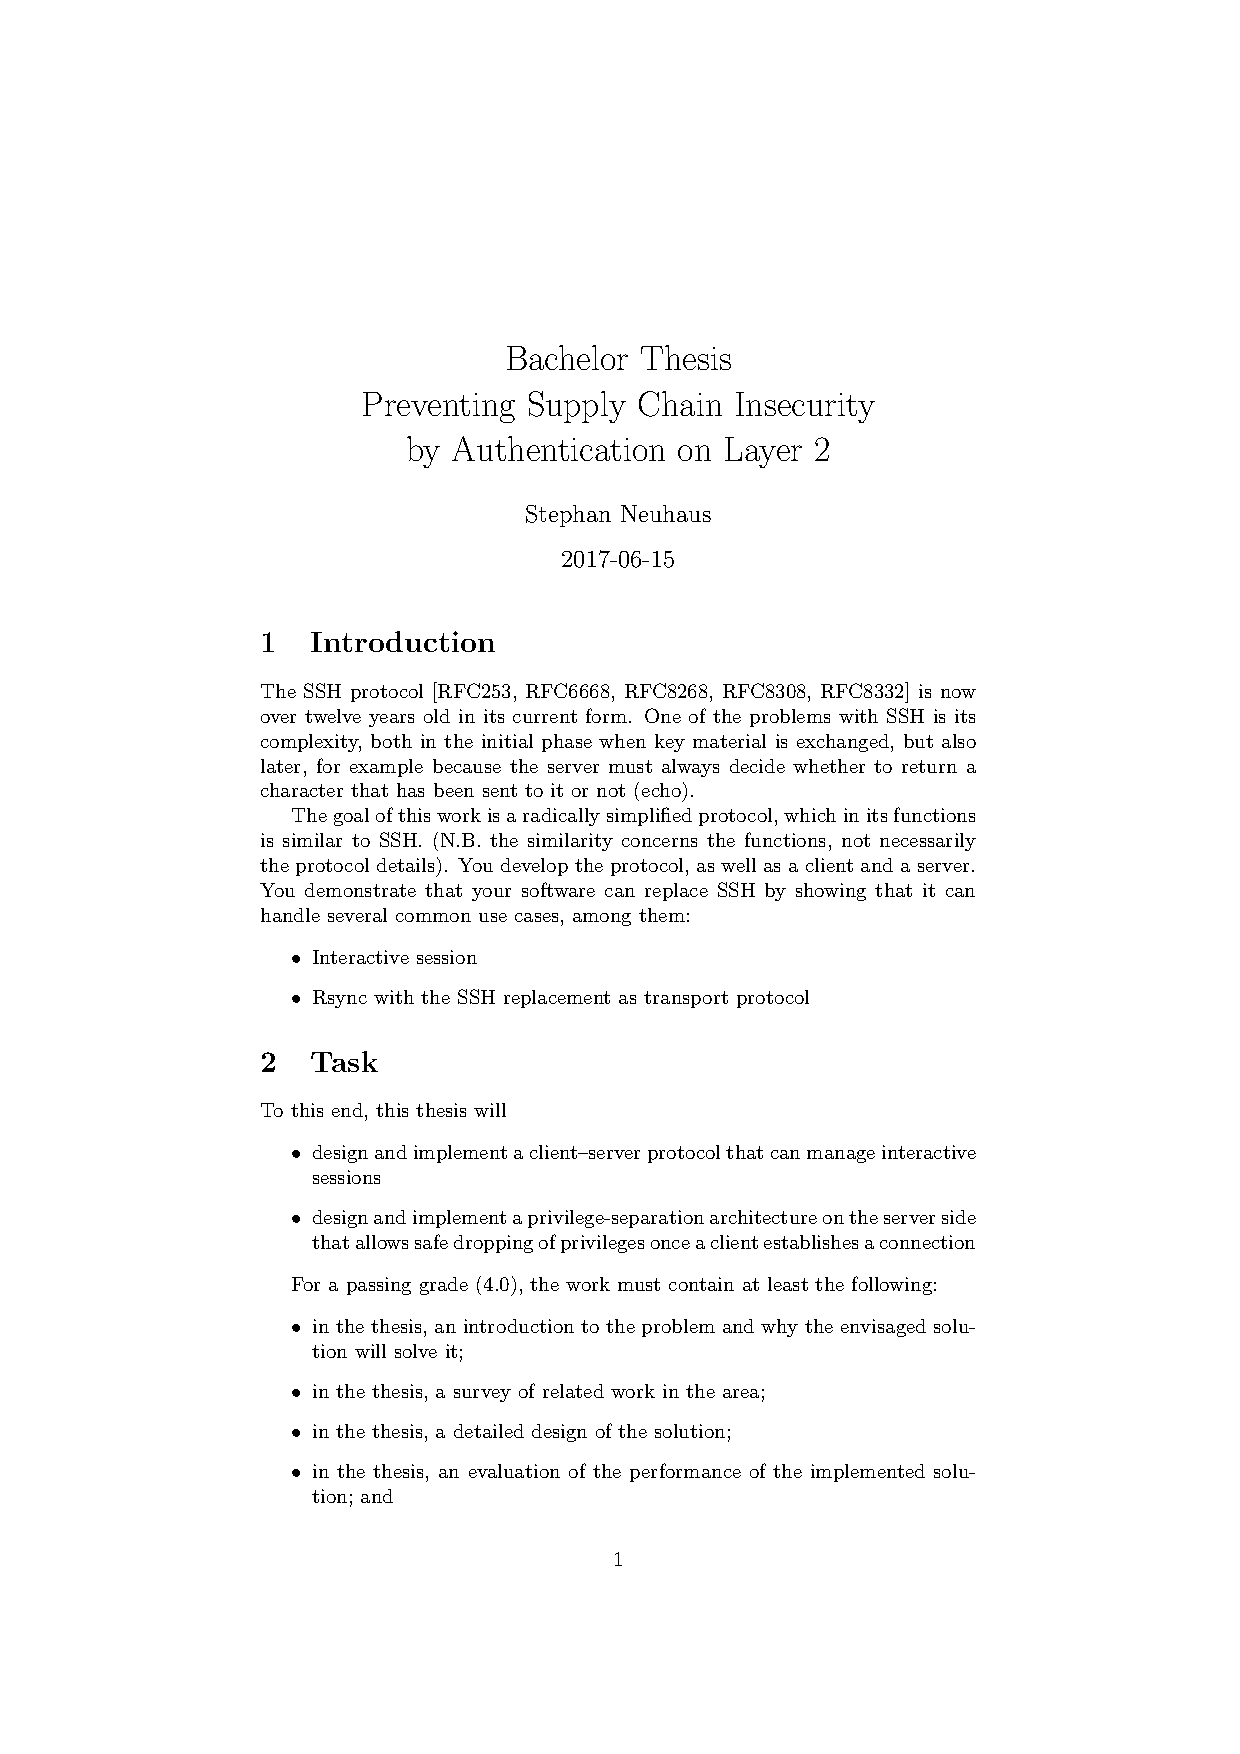
\includepdf[pages=-]{tasks.pdf}
\subsection{Project Plan}\label{ssec:ProjectPlan}
\includepdf[pages=-]{projectplan/Revised_project_plan.pdf}
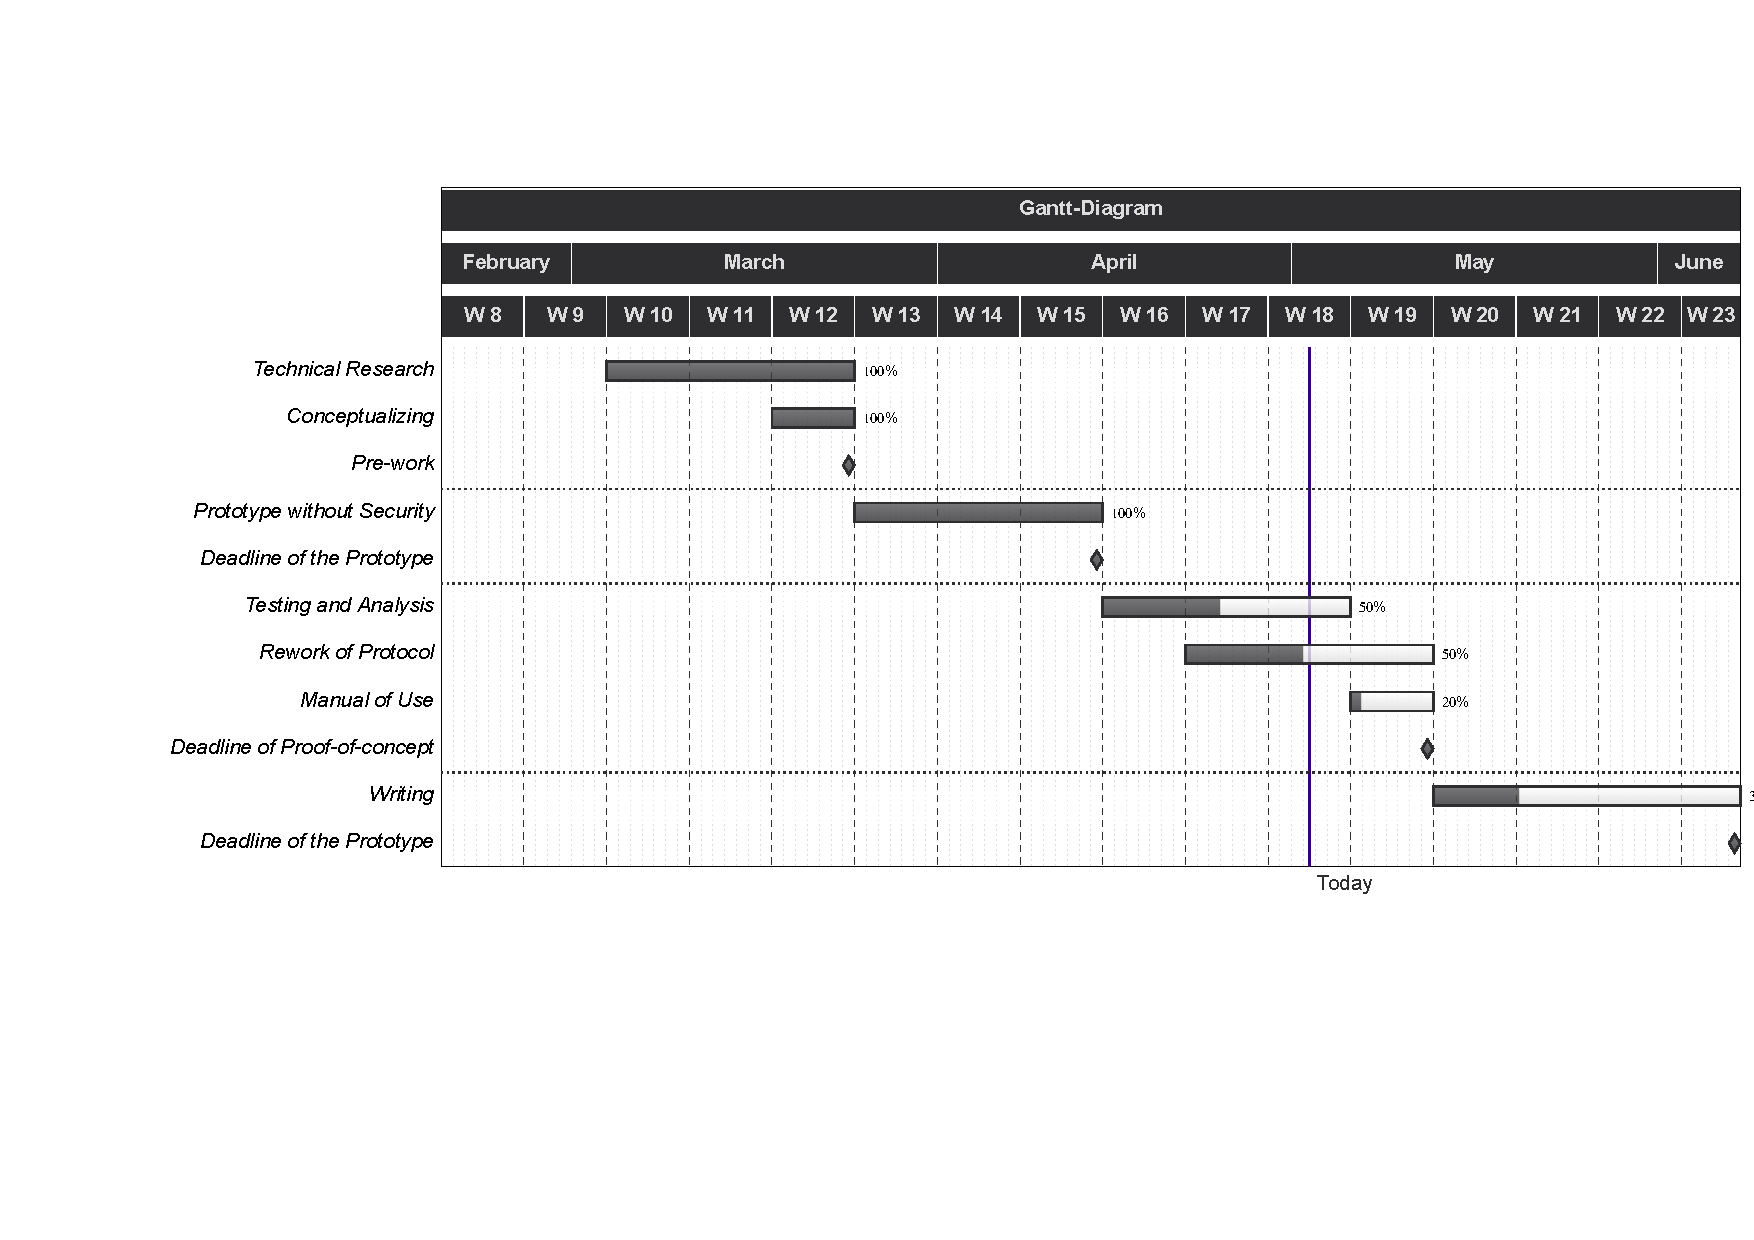
\includepdf[pages=-,landscape=true]{zhawGanttDiagram.pdf}
\subsection{Meeting Minutes}\label{ssec:MeetingMinutes}
The meeting minutes have a disruption in style and execution beginning from the 6th meeting.
Reason for this is because in the beginning of the project, Mr Schwarz was responsible for keeping the minutes, but he opted out of the project.
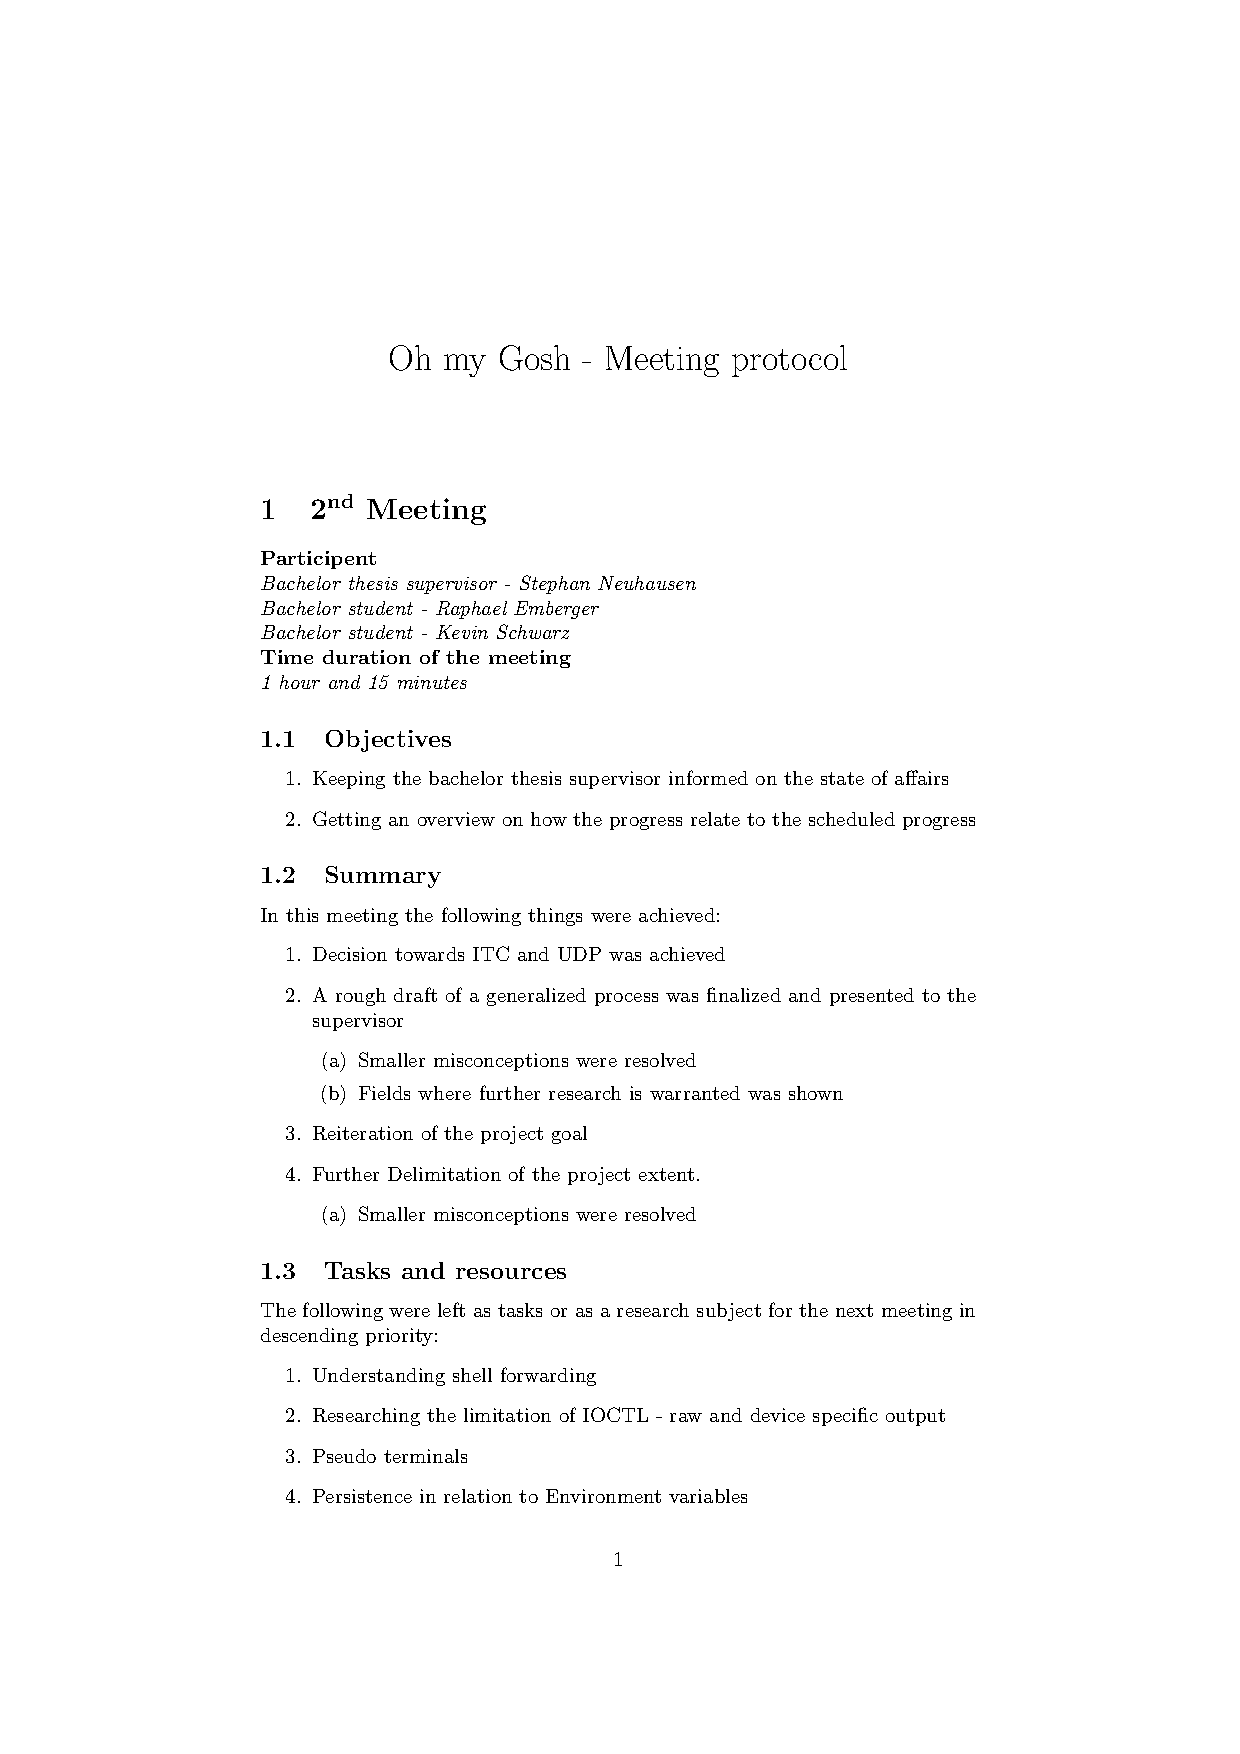
\includepdf[pages=-]{minutes/2nd_Meeting.pdf}
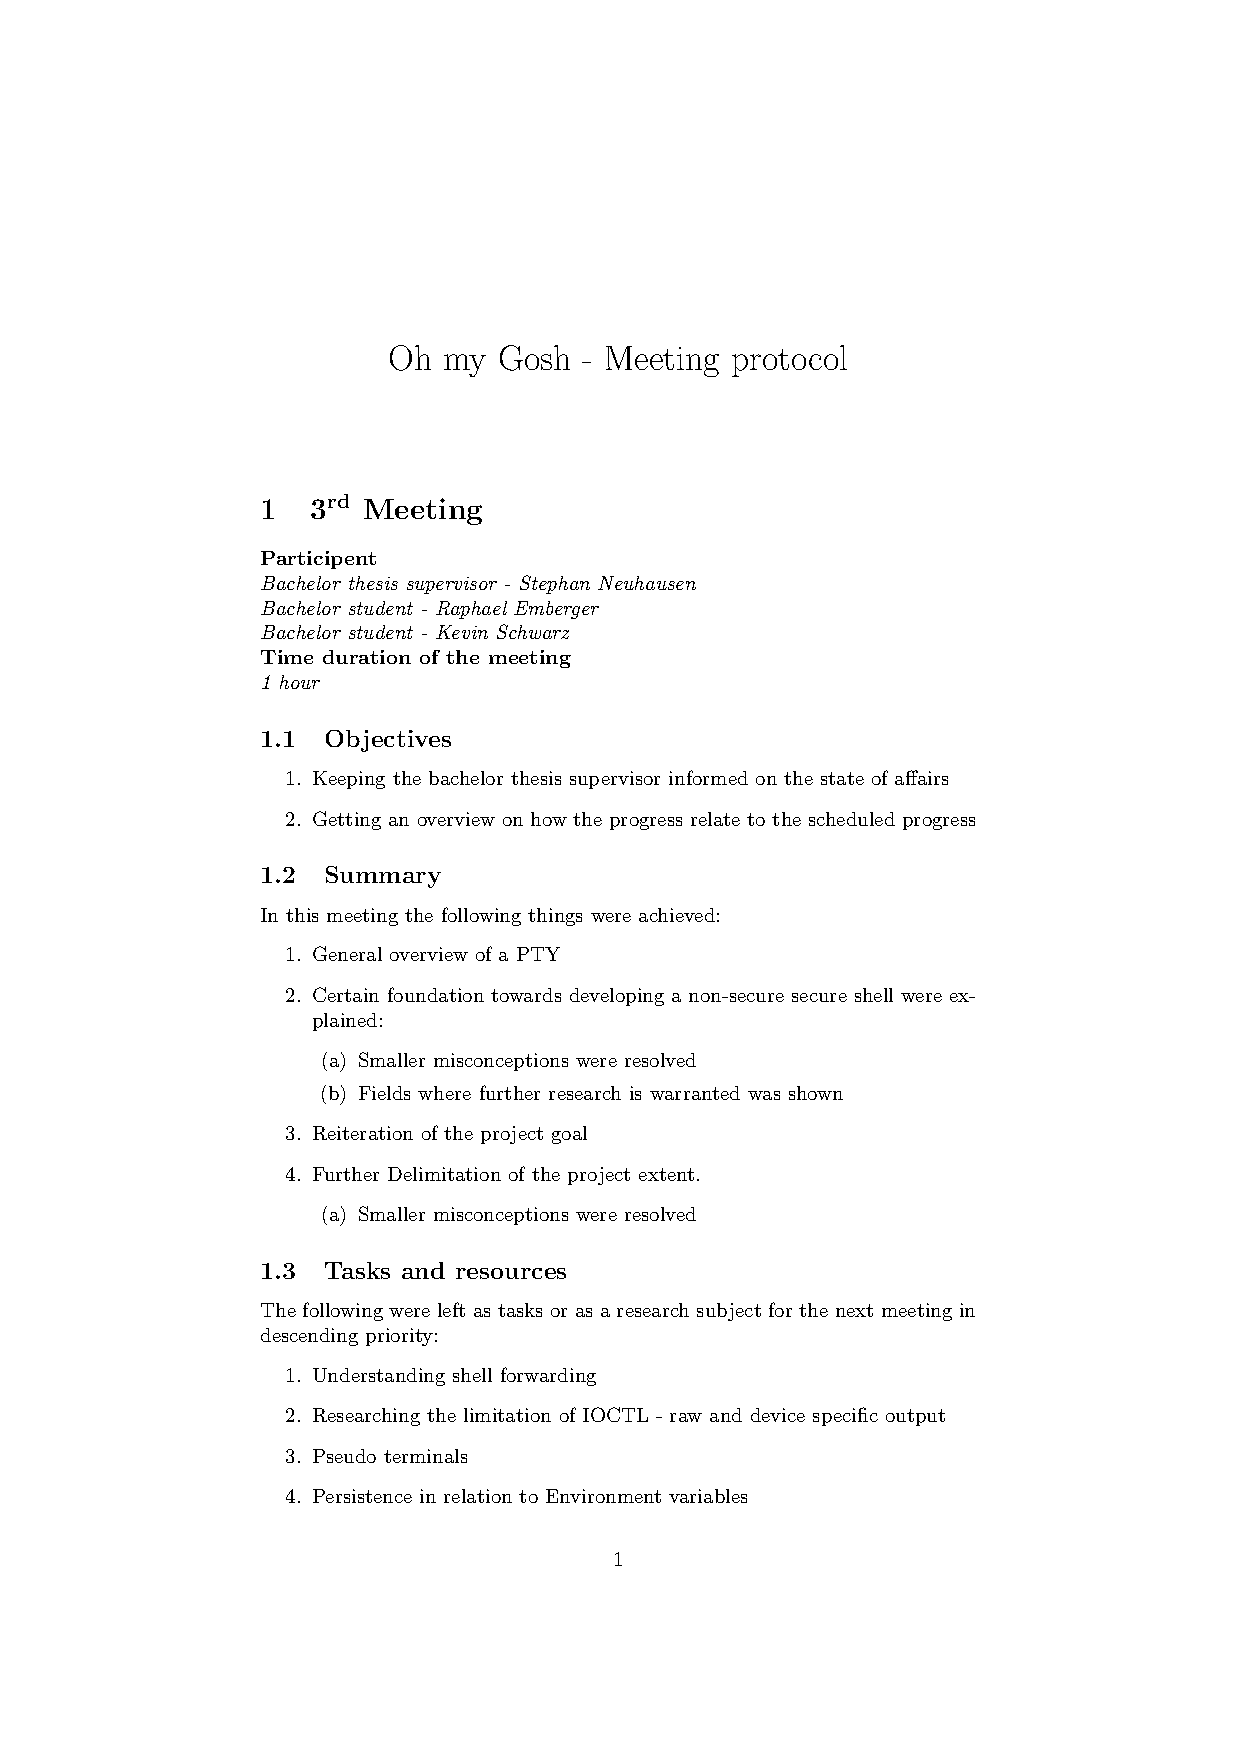
\includepdf[pages=-]{minutes/3rd_Meeting.pdf}
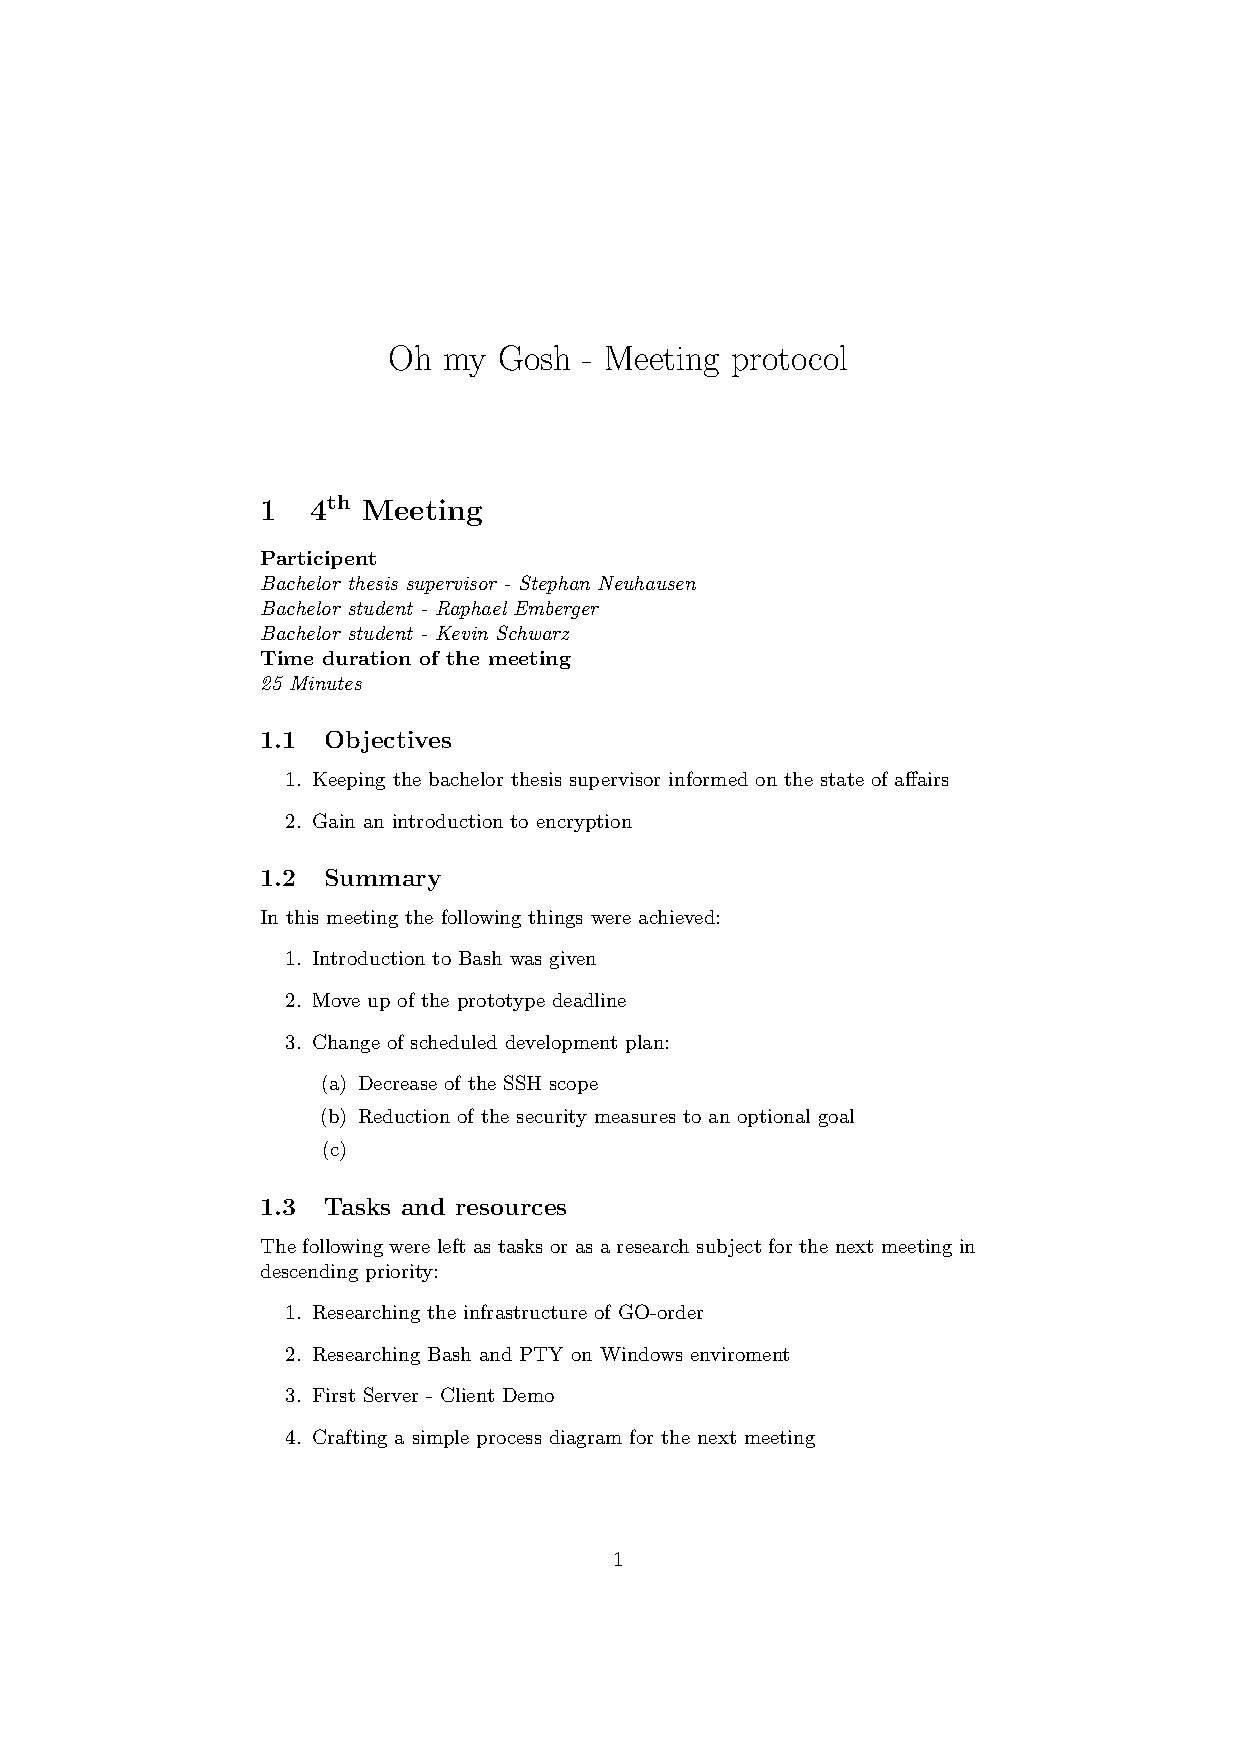
\includepdf[pages=-]{minutes/4th_Meeting.pdf}
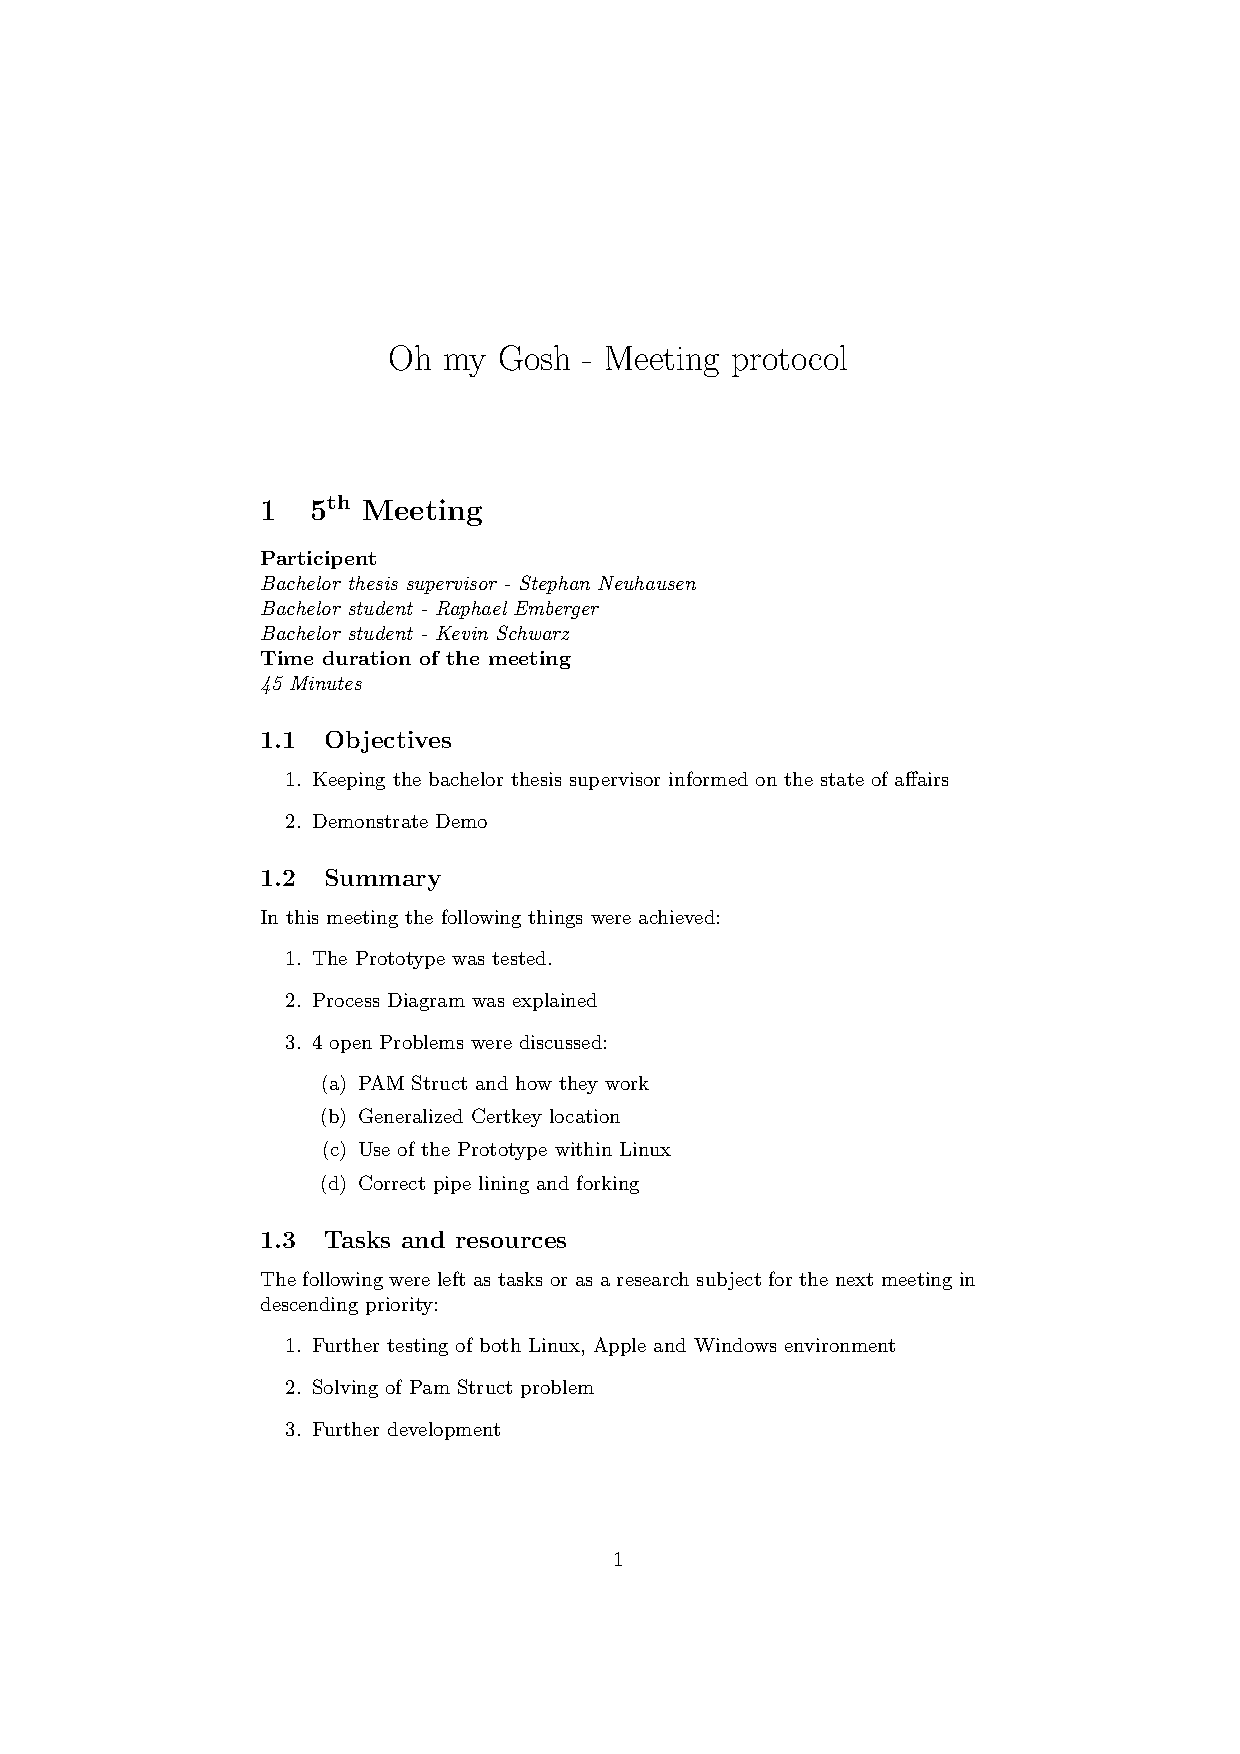
\includepdf[pages=-]{minutes/5th_Meeting.pdf}

\includepdf[pages=-]{minutes/6th_Meeting.pdf}

\includepdf[pages=-]{minutes/7th_Meeting.pdf}

\includepdf[pages=-]{minutes/8th_Meeting.pdf}

\includepdf[pages=-]{minutes/9th_Meeting.pdf}

\includepdf[pages=-]{minutes/10th_Meeting.pdf}
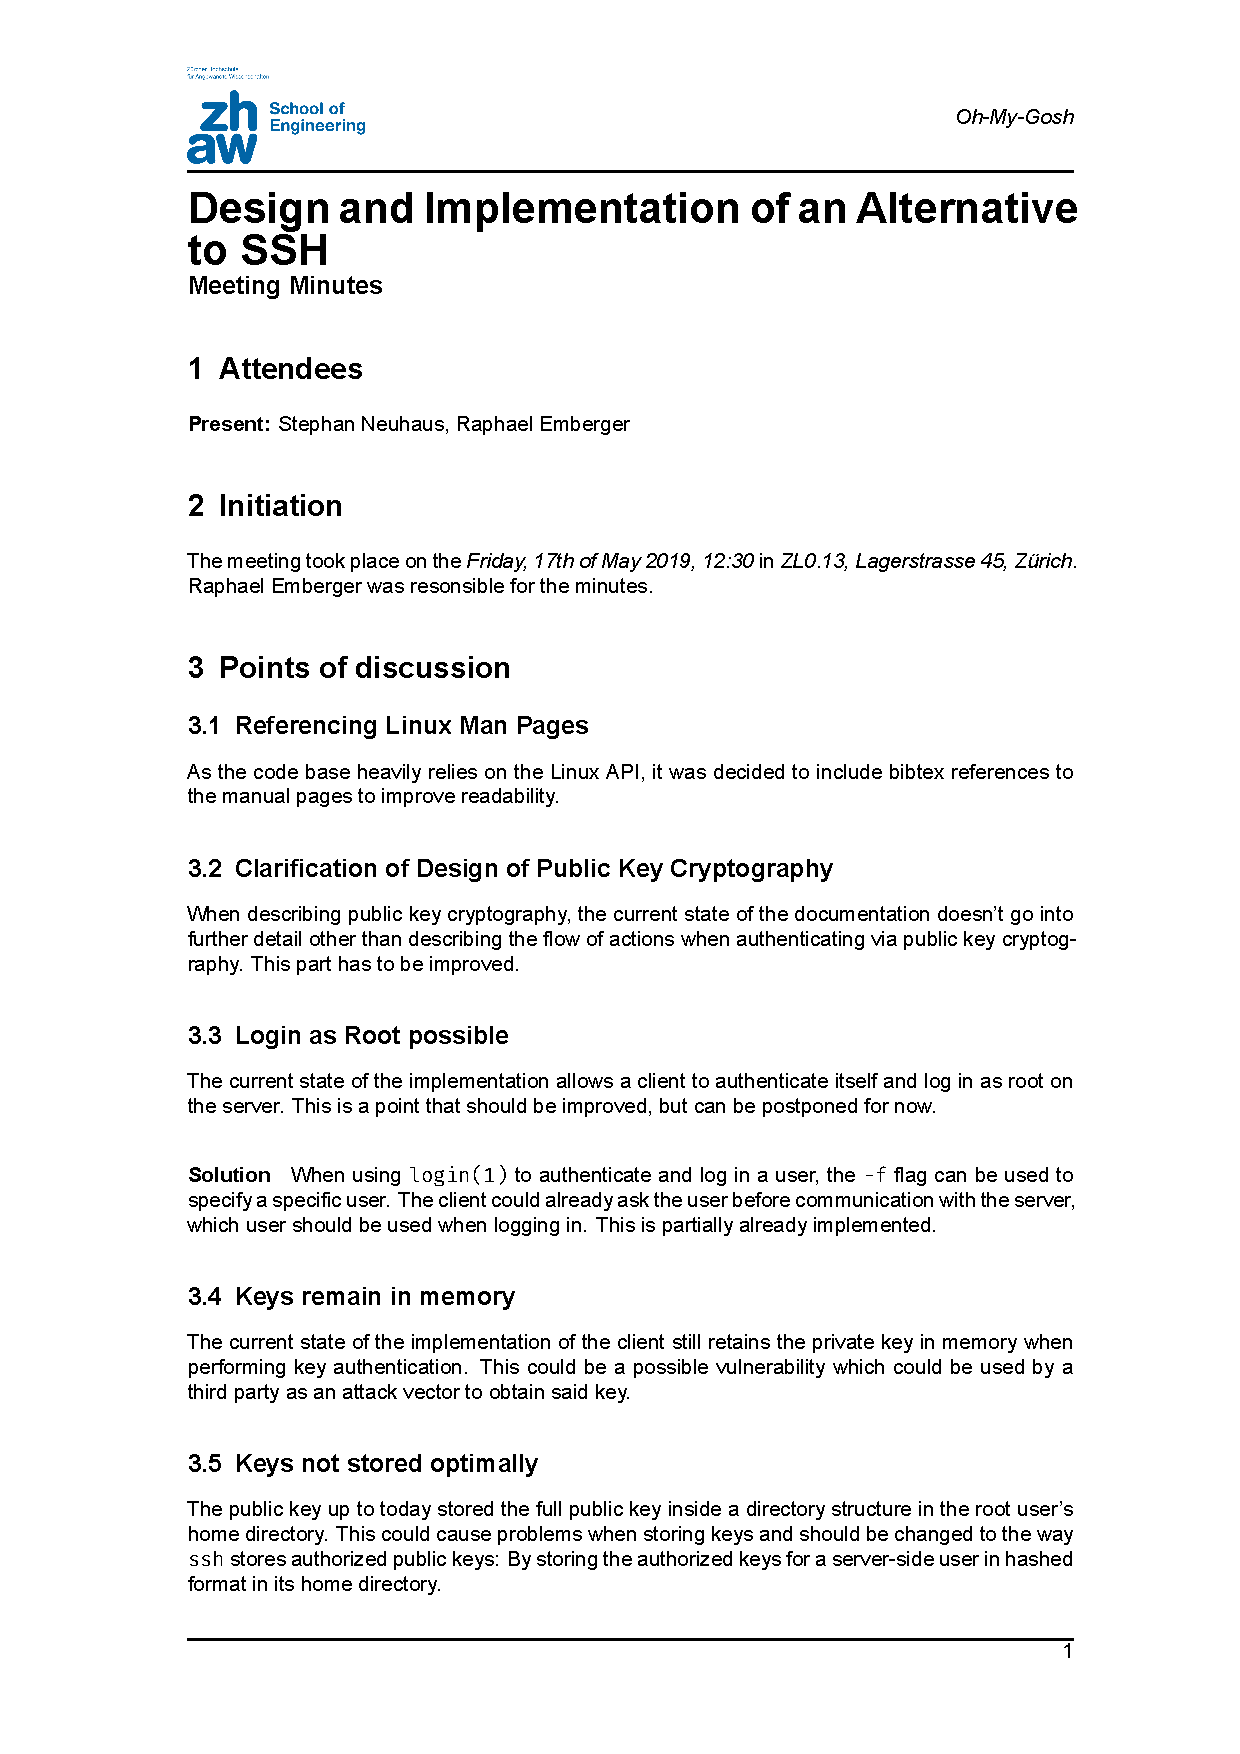
\includepdf[pages=-]{minutes/11th_Meeting.pdf}

\includepdf[pages=-]{minutes/12th_Meeting.pdf}

\section{Others}\label{sec:Others}
% CD mit dem vollständigen Bericht als pdf-File inklusive Film- und Fotomaterial
% (Schaltpläne und Ablaufschemata)
% (Spezifikationen u. Datenblätter der verwendeten Messgeräte und/oder Komponenten)
% (Berechnungen, Messwerte, Simulationsresultate)
% (Stoffdaten)
% (Fehlerrechnungen mit Messunsicherheiten)
% (Grafische Darstellungen, Fotos)
% (Datenträger mit weiteren Daten(z.B. Software-Komponenten) inkl. Verzeichnis der auf diesem Datenträger abgelegten Dateien)
% (Softwarecode)
Please refer to the USB-stick that has been handed in with this thesis.
The Git repository for the code (private) is located at:
\url{https://github.engineering.zhaw.ch/neut/oh-my-gosh}
and the documentation (clear-net) at:
\url{https://github.engineering.zhaw.ch/neut/oh-my-gosh-bericht}.

\end{document}
